\documentclass{article}
\usepackage[T1]{fontenc}
\usepackage{iclr2027_conference,times}
\usepackage{amsmath,amssymb,amsthm,mathtools}
\usepackage{graphicx,booktabs,microtype,float}
\usepackage{hyperref,url}
\usepackage{etoolbox}
\hypersetup{hidelinks}
\makeatletter
\patchcmd{\@maketitle}{Under review as a conference paper at ICLR 2027}{Research draft in ICLR 2027 format; not submitted}{}{\errmessage{Draft header patch failed}}
\patchcmd{\@maketitle}{Paper under double-blind review}{Research draft; not submitted}{}{\errmessage{Draft author patch failed}}
\makeatother
\newtheorem{theorem}{Theorem}
\newtheorem{proposition}[theorem]{Proposition}
\newtheorem{lemma}[theorem]{Lemma}
\newtheorem{corollary}[theorem]{Corollary}
\newcommand{\E}{\mathbb E}
\newcommand{\R}{\mathbb R}
\newcommand{\Var}{\operatorname{Var}}
\newcommand{\Cov}{\operatorname{Cov}}
\newcommand{\Normal}{\mathcal N}
\newcommand{\Uest}{\mathrm U}
\title{Integrability of Subsampled Compositional Diffusions}
\author{Anonymous authors}
\begin{document}
\maketitle

\begin{abstract}
Compositional diffusion inference combines many factor scores, making subsampling attractive when evaluating every factor is expensive. For a Feynman--Kac correction, however, an unbiased estimate of the instantaneous potential is exponentiated to obtain a positive particle weight. We study whether the resulting population operator has a finite normalizing constant. For Gaussian factors sampled with replacement, we give an exact reachable-variance recursion requiring only two extreme batches per step, independently of every finite batch size. A four-factor example has a finite full-factor update and an infinite subsampled normalizer for every finite batch size, even as local estimator mean squared error tends to zero. For sampling without replacement, an exact prefix/suffix recursion instead depends on batch size. An unbiased control preserves the deterministic quadratic tail of shared-component-covariance Gaussian mixtures, including noncommuting matrix tails, and hence the full-factor strict integrability domain. Combining this structure with classical Gaussian path twisting gives all fixed positive weight moments on a fixed finite grid. Oracle, learned-mixture and nonseparable sensing experiments separate these guarantees from accuracy and cost: certified methods can still fail against strong task-specific baselines, and finite high moments need not give useful finite-sample performance. The results identify tail curvature as a validity condition for exponential subsampling, alongside estimator variance and computational cost.
\end{abstract}

\section{Introduction}
Compositional inference combines separately available conditional distributions into a posterior for multiple observations or groups. It allows amortized factor models to be reused across datasets, including tall-data and hierarchical inference \citep{linhart2026,arruda2026}. Evaluating every factor score at each diffusion step can be expensive. Subsampling reduces this work, but the resulting weighted population update must first define a probability distribution.

For Feynman--Kac weighting, the correction is quadratic in the factor scores. A random batch gives a conditionally unbiased estimate, whose exponential is a positive weight. Yet a rare batch can create excessive positive quadratic growth in a Gaussian tail, making the population normalizer infinite. Finite particles can miss both the offending batch and the extreme states it affects. Local mean squared error and observed effective sample size consequently need not detect the failure.

We study this existence question for a specified weighted Euler discretization. It is distinct from intermediate-distribution mismatch and learned-score error \citep{linhart2026,soiffer2026}. For scalar Gaussian factors, an exact two-choice recursion replaces enumeration of every with-replacement batch history. Its decision is independent of every finite batch size. Without replacement, an exact prefix/suffix recursion instead depends on batch size. An affine control with the correct tail curvature preserves the full-factor strict domain; a vector envelope argument extends this property to noncommuting covariance matrices. Oracle, learned-density and nonseparable sensor studies then distinguish existence, finite-particle accuracy and computational value.

The contribution is a computable validity analysis of exponential factor subsampling. The experiments test its implications and its limits. Strong baselines exploit product structure when available and use direct-likelihood SMC when the observation model permits it. A certificate of existence is evaluated separately from any speed--accuracy claim.

\section{Compositional flow and random exponential weights}
Let $\varphi$ be the standard Gaussian density on $\R^d$. Factor density $q_{g,0}$ evolves under the variance-preserving Ornstein--Uhlenbeck process
\begin{equation}
 dX_u=-\tfrac12X_u\,du+dW_u,\qquad
 X_u=e^{-u/2}X_0+\sqrt{1-e^{-u}}\,\xi.
\end{equation}
Write $s_g(x,u)=\nabla\log q_{g,u}(x)$, $r_g=s_g+x$, and $R=\sum_{g=1}^G r_g$. The unnormalized compositional path is
\begin{equation}\label{eq:path}
 \rho_u(x)=\varphi(x)^{1-G}\prod_{g=1}^Gq_{g,u}(x),\qquad
 \nabla\log\rho_u=-x+R.
\end{equation}
We assume this path is integrable over the interval considered. With reverse time $t=U-u$, define
\begin{equation}\label{eq:drift-potential}
 b_\kappa(x,u)=\frac{1+\kappa}{2}R(x,u)-\frac\kappa2x,
 \qquad
 g(x,u)=\frac12\left(\|R(x,u)\|^2-\sum_{g=1}^G\|r_g(x,u)\|^2\right),
\end{equation}
where $\kappa>0$. Direct differentiation gives
\begin{equation}\label{eq:fk}
 -\partial_u\rho_u=-\nabla\cdot(b_\kappa\rho_u)+\frac\kappa2\Delta\rho_u+g\rho_u.
\end{equation}
Thus the normalized continuous flow is represented by a Feynman--Kac diffusion whenever its required moments exist. Appendix~\ref{app:flow} derives this identity. Our results concern the following discrete operator; they do not assert that its finite-step target equals $\rho_0$.

For a step $h>0$ at level $u$, independently draw a batch $B=(I_1,\ldots,I_M)$, with each index uniform on $\{1,\ldots,G\}$. For $M\ge2$, define
\begin{align}
 \widehat R_B&=\frac GM\sum_{i=1}^M r_{I_i},\label{eq:Rhat}\\
 \widehat g_{\Uest,B}&=\frac12\left\{
 \frac{G^2}{M(M-1)}\sum_{i\ne j}r_{I_i}^{\mathsf T}r_{I_j}
 -\frac GM\sum_i\|r_{I_i}\|^2\right\}.\label{eq:U}
\end{align}
Both are conditionally unbiased at every fixed $(x,u)$. The plug-in estimator $\widehat g_{\mathrm N}=\tfrac12(\|\widehat R\|^2-\tfrac GM\sum_i\|r_{I_i}\|^2)$ is also considered. Its conditional bias is $G^2\operatorname{tr}\Cov_I(r_I)/(2M)$.

For either estimator, let $\widehat b_B=(1+\kappa)\widehat R_B/2-\kappa x/2$. The positive kernel and its normalized update are
\begin{equation}\label{eq:kernel}
 Q_{u,h}f(x)=\E_{B,\xi}\!\left[e^{h\widehat g_B(x,u)}
 f\!\left(x+h\widehat b_B(x,u)+\sqrt{\kappa h}\,\xi\right)\right],
 \qquad \Phi_{u,h}(\eta)(f)=\frac{\eta Q_{u,h}f}{\eta Q_{u,h}1}.
\end{equation}
The denominator must belong to $(0,\infty)$. Conditional unbiasedness of $\widehat g$ does not imply $\E_B e^{h\widehat g}=e^{hg}$ or that $\eta Q1$ is finite. We analyze this denominator before making any particle-convergence claim.

\section{Gaussian integrability certificates}
In one dimension, Gaussian factors have $r_g(x,u)=-a_g(u)x+d_g(u)$. At a fixed level, suppress $u$ and suppose $a_g\ge0$. For a batch, put $m=M^{-1}\sum_i a_{I_i}$ and $s^2=M^{-1}\sum_i(a_{I_i}-m)^2$. The drift and potential have the form
\begin{equation}\label{eq:quadratic}
 \widehat b_B(x)=-\tfrac12((1+\kappa)\widehat A_B+\kappa)x+\text{constant},
 \qquad \widehat g_B(x)=\widehat c_Bx^2+\text{linear terms},
\end{equation}
where $\widehat A_B=Gm$, and
\begin{equation}\label{eq:batch-c}
 \widehat c_{\Uest,B}=\frac12\left[G(G-1)m^2-
 \left(\frac{G^2}{M-1}+G\right)s^2\right],\qquad
 \widehat c_{\mathrm N,B}=\frac12[G(G-1)m^2-Gs^2].
\end{equation}
For the full-factor update, $A=\sum_g a_g$ and $c=(A^2-\sum_g a_g^2)/2$.

\begin{lemma}[Conditional Gaussian update]\label{lem:gaussian}
Suppose the normalized state conditional on a batch history is Gaussian with variance $V>0$. Its next conditional normalizer is finite if and only if
\begin{equation}\label{eq:D}
 D_B(V)=1-2h\widehat c_B V>0.
\end{equation}
When finite, the propagated conditional law is Gaussian with variance
\begin{equation}\label{eq:variance}
 F_B(V)=\frac{[1-h((1+\kappa)\widehat A_B+\kappa)/2]^2 V}{D_B(V)}+\kappa h.
\end{equation}
The criterion and variance are independent of the Gaussian mean and the linear terms in the potential.
\end{lemma}
\begin{proof}
Multiplication by the weight changes the Gaussian precision from $V^{-1}$ to $V^{-1}-2h\widehat c_B$. A nonpositive precision gives an infinite integral on $\R$, including the zero-precision case. For positive precision, completing the square gives tilted variance $V/D_B(V)$. The affine Euler map and independent Gaussian noise give \eqref{eq:variance}.
\end{proof}

Every batch history has positive probability. If one of its conditional normalizers is infinite, Tonelli's theorem makes the joint nonnegative integral infinite. If all histories remain finite for a finite number of steps, their finite sum is finite. A direct check appears to require exponentially many histories. The following result removes that enumeration.

\begin{theorem}[Two extreme batches suffice]\label{thm:extreme}
Fix a finite time grid, $G\ge2$, $M\ge2$, and $\kappa>0$. Assume scalar Gaussian factors with $a_g(u_k)\ge0$ and an initial Gaussian variance $V_0>0$. For either estimator in \eqref{eq:batch-c}, set $V_{\max,0}=V_0$. At step $k$, let $a_-=\min_g a_g(u_k)$, $a_+=\max_g a_g(u_k)$ and define, for $z\in\{a_-,a_+\}$,
\begin{equation}\label{eq:extreme-recursion}
 D_z=1-h_kG(G-1)z^2V_{\max,k},\qquad
 F_z=\frac{[1-h_k((1+\kappa)Gz+\kappa)/2]^2V_{\max,k}}{D_z}+\kappa h_k.
\end{equation}
If some $D_z\le0$, the population normalizer is infinite at this step. Otherwise set $V_{\max,k+1}=\max(F_{a_-},F_{a_+})$ and continue. Until failure, this is exactly the largest reachable conditional variance. Consequently the integrability decision is identical for every finite $M\ge2$, for both the plug-in and unbiased estimators.
\end{theorem}
\begin{proof}
Both coefficients in \eqref{eq:batch-c} are at most $G(G-1)m^2/2$, with equality for a constant batch. Since $0\le m\le a_+$, a nonpositive denominator can occur if and only if it occurs for the constant strongest-factor batch at the largest reachable variance. On the common positive-denominator domain, $F_B(V)$ is nondecreasing in $V$ and in $\widehat c_B$ with $\widehat A_B$ fixed. It remains to maximize
\[
 f(m)=\frac{V[1-h((1+\kappa)Gm+\kappa)/2]^2}{1-hVG(G-1)m^2},\quad m\in[a_-,a_+].
\]
This function is convex. Indeed, with affine $n(m)=\sqrt V[1-h((1+\kappa)Gm+\kappa)/2]$ and positive concave $d(m)=1-hVG(G-1)m^2$,
\[
 f(m)=\sup_{z\in\R}\{2zn(m)-z^2d(m)\},
\]
the supremum of convex quadratics. Its maximum on the interval occurs at an endpoint. The corresponding constant batches exist for every $M$ and have positive probability. Induction establishes attainability of each maximum and the stated decision.
\end{proof}

The cost is $O(KG)$ to obtain the extrema and $O(K)$ scalar transitions, with no enumeration over $G^M$ batches. For diagonal product factors, apply the recursion to each coordinate: a single failing coordinate suffices for divergence, while positivity for every coordinate certifies every history.

\paragraph{Uniform sampling without replacement.}
For a uniform subset $S$ of size $2\le M\le G$, the unbiased potential is $G(G-1)\sum_{i<j,\,i,j\in S}r_i^{\mathsf T}r_j/[M(M-1)]$. Its exact Gaussian certificate depends on $M$. After sorting $a_1\le\cdots\le a_G$, only the $M+1$ subsets containing the $j$ weakest and $M-j$ strongest factors, $0\le j\le M$, need be checked. Fixing all but one selected strength makes the drift and quadratic potential coefficients affine in the remaining strength; convexity of the squared-affine-over-positive-affine variance map permits an endpoint exchange. Repeated exchanges give these prefix/suffix subsets. Appendix~\ref{app:without-replacement} gives the full theorem and multi-step proof. At $M=G$, this update is the full-factor operator.

\subsection{An exact four-factor separation}
Take zero-mean Gaussian factor precisions $1+\lambda_g$ with $\lambda=(1/10,1/5,2,4)$. At $u=\log2$, the residual precisions are $a=(1/21,1/11,1/2,2/3)$. The normalized compositional density is $\Normal(0,V)$ with $V=154/355$. For $h=1/2$ and $\kappa=1$,
\begin{equation}\label{eq:counterexample}
 A=\frac{201}{154},\quad c=\frac{346}{693},\quad
 D_{\mathrm{full}}=\frac{2503}{3195}>0,\qquad
 D_{\mathrm{all\ strongest}}=-\frac{167}{1065}<0.
\end{equation}
The all-strongest batch occurs with probability $4^{-M}$ and has $\widehat c=8/3$ for either estimator. Thus the subsampled normalizer is infinite for every finite $M$, whereas the full-factor update has log normalizer $-\tfrac12\log(2503/3195)$ and output variance
\begin{equation}
 [1-\tfrac12(A+\tfrac12)]^2\frac{154/355}{2503/3195}+\tfrac12.
\end{equation}
At each fixed state, both unbiased estimators converge in mean square as $M\to\infty$, because the index distribution has finite support. Their state-averaged mean squared errors also vanish for this Gaussian input. This limit does not interchange with the nonnegative exponential integral. For $P$ independent particle batches, the probability of observing at least one all-strongest batch is $1-(1-4^{-M})^P$; observing such a batch still does not guarantee an extreme sampled state.

\section{Preserving the deterministic quadratic tail}
Suppose each scalar factor is a finite Gaussian mixture whose components share variance $v_g$ but may have different means. After forward noising, its residual score admits
\begin{equation}\label{eq:tail-decomposition}
 r_g(x,u)=r_g^0(x,u)+e_g(x,u),\qquad
 r_g^0=-a_g(u)x+d_g(u),\qquad \sup_x|e_g(x,u)|<\infty,
\end{equation}
where $a_g(u)=[1-e^{-u}+e^{-u}v_g]^{-1}-1$. One may use $d_g=e^{-u/2}\bar\mu_g/[1-e^{-u}+e^{-u}v_g]$, with $\bar\mu_g$ the mixture mean. The bound follows because the posterior component mean lies in the convex hull of finitely many component means. A Gaussian fit using the total mixture variance generally does not satisfy this bounded-residual property.

Write $R_0=\sum_g r_g^0$ and $Q_0=\sum_g\|r_g^0\|^2$. Compute both affine/quadratic functions exactly. The tail-control estimator is
\begin{align}\label{eq:tail-estimator}
 \widehat R_{\mathrm T}&=R_0+\frac GM\sum_i e_{I_i},\\
 \widehat g_{\mathrm T}&=\tfrac12(\|R_0\|^2-Q_0)
 +R_0^{\mathsf T}\frac GM\sum_i e_{I_i}
 -\frac GM\sum_i(r_{I_i}^0)^{\mathsf T}e_{I_i}\nonumber\\
 &\hspace{8mm}+\frac12\left\{\frac{G^2}{M(M-1)}\sum_{i\ne j}e_{I_i}^{\mathsf T}e_{I_j}-\frac GM\sum_i\|e_{I_i}\|^2\right\}.\nonumber
\end{align}
Taking conditional expectations proves unbiasedness. Expanding $r_g=r_g^0+e_g$ gives exactly the full potential. Moreover, every batch has the same quadratic coefficient $c$ and the same linear drift coefficient as the full-factor construction; all random contributions to the potential grow at most linearly.

\begin{theorem}[Strict integrability domain of tail control]\label{thm:tail}
Consider scalar equal-component-variance Gaussian mixture factors, a finite grid with $\kappa>0$, and an initial density satisfying
\begin{equation}\label{eq:envelope}
 \log p_0(x)=-x^2/(2V_0)+O(1+|x|).
\end{equation}
At each step propagate the full-factor quadratic variance using \eqref{eq:variance} with $(A,c)$. If all resulting denominators are strictly positive, both the full-factor and tail-control population normalizers are finite. If the first nonpositive denominator is strictly negative, both normalizers are infinite there. This statement holds for every finite $M\ge2$. No claim is made at a zero denominator for general mixtures.
\end{theorem}
\begin{proof}
For a density with \eqref{eq:envelope} and a potential $cx^2+O(1+|x|)$, weighting replaces its quadratic variance by $V/(1-2hcV)$ when the denominator is positive; a negative denominator forces an infinite integral. An affine map plus a bounded displacement followed by independent Gaussian noise preserves the quadratic-tail form, with variance \eqref{eq:variance}; Appendix~\ref{app:envelope} proves this step. Equation~\eqref{eq:tail-estimator} makes these quadratic coefficients common to every batch. Induction over the finite histories gives the result.
\end{proof}

The theorem certifies existence of the discretized population flow. It does not remove Euler error or the effect of exponentiating the bounded residual estimator. Its computational requirement is also explicit: the affine coefficient sums can be prepared once per time level in $O(Gd)$ work, followed by $M$ nonlinear factor evaluations per particle. The control requires known component tail variances, which limits its direct applicability to arbitrary learned score models.

More generally, an arbitrary affine control also admits an exact strict-domain certificate: it suffices to evaluate the $G$ constant batches, each containing one repeated factor. Appendix~\ref{app:general-control} proves this extension and shows that the paired correction has the same strict integrability domain. Thus the moment-matched and tail-matched controls in our experiments can be classified using the same test, although only the latter preserves the full-factor domain by construction.

\paragraph{Noncommuting covariance matrices.}
For shared-component-covariance mixtures on $\R^d$, write $r_g=-A_gx+O(1)$ with $A_g=A_g^{\mathsf T}$. Set $A_\Sigma=\sum_gA_g$, $C=(A_\Sigma^{\mathsf T}A_\Sigma-\sum_gA_g^{\mathsf T}A_g)/2$ and $L=I-h((1+\kappa)A_\Sigma+\kappa I)/2$. The scalar strict-domain test becomes
\[
H=V^{-1}-2hC\succ0,\qquad V^+=LH^{-1}L^{\mathsf T}+\kappa hI.
\]
An incoming log density $-x^{\mathsf T}V^{-1}x/2+O(1+\|x\|)$ retains this form after a finite update. A negative eigenvalue of $H$ forces divergence, while the semidefinite boundary remains unclassified. Deterministic tail control shares these matrices with full weighting. Appendix~\ref{sec:matrix-tail-extension} proves the vector envelope result, including singular $L$. This extension concerns common tail coefficients; the scalar extreme-batch reduction is not used for general random matrices.

\paragraph{Anchoring the bounded remainder.}
Preserving curvature leaves freedom in the affine intercept. Given a deterministic point $x_\star(u)$, set $r_g^0(x,u)=-A_g(u)x+d_g^\star(u)$ with
\[
d_g^\star(u)=r_g(x_\star(u),u)+A_g(u)x_\star(u).
\]
Every residual then vanishes at the anchor, while remaining bounded over the state space. The drift and potential estimators are conditionally exact at that point. Away from it, their variances and exponential bias remain nonzero. This construction uses the known tail curvature, with an intercept selected from factor scores; it is a control-variate realization related to gradient anchoring in stochastic-gradient MCMC \citep{baker2019}.

For the diagonal learned experiment, we initialize the anchor at the affine composed-score root and use six fixed Newton updates. The denominator is bounded below by $0.2$, and each coordinate update is clipped to $[-1,1]$. The nonseparable experiment uses the corresponding full Hessian, with eigenvalues bounded below by $0.2$ and an update norm at most one. These choices are fixed before development. Preparation uses only factor parameters and time, with seven residual and six derivative evaluations per factor and time level. No reference posterior or true state enters it. Preparation and device transfers are included in reported sampling time.


\paragraph{From existence to finite weight moments.}
Tail control also gives a tractable proposal construction. Absorb the deterministic quadratic potential into its Gaussian path law using classical backward twisting \citep{whiteley2014,heng2020}, and correct both the remaining potential and the transition density. For a fixed finite grid in the strict domain, the complete log density correction grows at most linearly in the path norm. Consequently every fixed positive importance-weight moment is finite (Theorem~\ref{thm:gaussian-twist-moments}). This preserves the specified discrete random-kernel target, including its possible discrepancy from the full-factor or continuous posterior. The guarantee applies to independent paths; it supplies neither a uniform-in-time bound nor a claim of small practical variance.

\section{Experiments}\label{sec:experiments}
\paragraph{Evidence design.}
Oracle Gaussian and mixture factors isolate subsampling from score learning. Five mixture density networks then test compositions of learned conditional densities with known Gaussian tails. Each network completes 40,000 training updates; reference posterior labels are not used for training. A third family has nonorthogonal observations and analytically available nonseparable posterior mixtures. Sampling time includes method-specific preparation, transfer and resampling. One-time prediction of learned factor parameters and construction of common reference distributions are reported separately. The networks are evaluated once per dataset; subsequent factor scores are analytic mixture calculations.

\subsection{Finite samples can conceal a divergent population update}
In the four-factor example of \eqref{eq:counterexample}, every finite with-replacement batch size has an infinite normalizer. With $1{,}048{,}576$ particles, increasing $M$ from 2 to 32 nevertheless lowers mean potential MSE from $0.46798$ to $0.01857$ and increases median ESS fraction from $0.000424$ to $0.932706$. At $M=32$, all 20 runs miss the nonintegrable batch events. The observed mean log normalizer is $0.126047$ with standard deviation $0.000259$, close to the exact full-factor value $0.122049$. The theorem supplies the divergence statement; finite observations illustrate its limited visibility.

\begin{figure}[t]
\centering
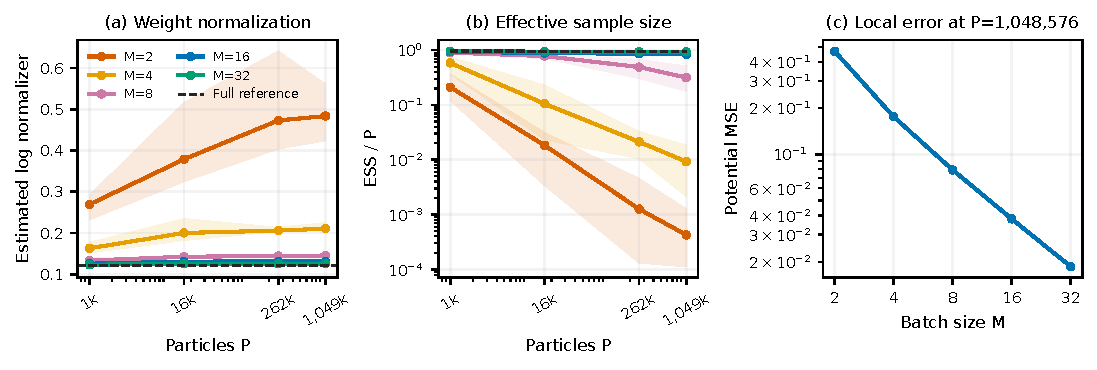
\includegraphics[width=\linewidth]{figures/one_step.pdf}
\caption{The exact divergence certificate is unchanged as batch size grows. Finite-particle normalizer estimates and ESS can nevertheless appear stable. Panels show medians and interquartile ranges over 20 runs, with mean potential MSE and one standard deviation at the largest particle count.}
\label{fig:paper-one-step}
\end{figure}

The full-factor Euler scheme also has a finite-step boundary. At $G=64,K=128$, the ordinary Gaussian benchmark has a negative denominator, while observed eight-dimensional W1 is only $0.0176$. Conversely, finite configurations can have substantial particle error. For a separate 16-step Gaussian path, the exact first weight moment is finite and the second infinite (Appendix~\ref{app:dual-results}). Existence, second moments and observed error are separate diagnostics.

\subsection{Tail control and useful posterior accuracy}
The fixed benchmark includes 1,980 oracle cells, followed by 1,080 oracle-extension and 1,000 learned sampling cells. In the learned study, all 600 full or tail-controlled cells have finite normalizers; all 400 raw subsampled cells are divergent. The largest setting uses $G=64,d=8,N=32768,K=2048$. W1 against the learned composition is $0.0189$ for full weighting and $0.0907$ for fixed-mean tail control without replacement. Thus restoring the finite domain alone does not solve the accuracy problem.

Anchoring reduces this fixed-mean control error on a separately held-out cohort: W1 changes from $0.09539$ to $0.01967$, compared with full weighting at $0.01682$. An equivalent implementation takes $3.844$ seconds against $6.039$ for full weighting. Its W1 degradation upper bound is $0.00608$, exceeding the declared $0.002$ allowance. On the same saved particles, observed 90\% interval coverage improves from $66.00\%$ to $87.25\%$, with full weighting at $88.50\%$. These ten data seeds and five trained models do not establish general calibration. Appendix~\ref{app:dual-results} retains the complete-kernel correction ablations and all failed joint accuracy--cost criteria.

Product structure also matters. Coordinatewise full-factor SMC lowers W1 from $0.6973$ to $0.2703$ on the difficult product mixture; joint sign TV remains $0.3685$. This is a strong problem-specific baseline, with residual mode error. A fresh study uses eight development targets to select an anchored batch/particle/grid configuration and fixes it before evaluating five checkpoints crossed with twenty new datasets. The two-way paired bootstrap samples checkpoints and datasets separately. Results are assessed against both joint and coordinatewise full-factor baselines.

The selected configuration has $N=8192,K=1024,M=8$. On the 100 new model--dataset pairs, its W1 is $0.01908$ in $1.240$ seconds, compared with $0.01972$ in $6.097$ seconds for the original $N=32768,K=2048$ joint baseline. Its one-sided 95\% W1-degradation bound is $0.001323$, below the fixed $0.002$ allowance. Coordinatewise full weighting at the original budget achieves $0.01556$; the corresponding degradation bound is $0.005200$, so the predeclared requirement to pass both baselines fails.

A post-hoc same-cohort ablation gives both baselines the selected $N,K$ and replays the anchor. Full weighting then takes $1.404$ seconds at W1 $0.02076$, coordinatewise weighting $1.498$ seconds at $0.01667$, and the anchor $1.235$ seconds at $0.01908$. Thus the anchor's time reduction against joint weighting is about $12\%$ at equal particle/grid budgets; most of the apparent $4.9\times$ difference above is budget selection. Its W1-degradation upper bound against the matched coordinatewise baseline is $0.004199$, again exceeding $0.002$. This ablation reuses the same targets and supplies no additional independent data. Appendix~\ref{app:paper-level-results} gives the audit and intervals.

\subsection{A nonseparable inverse problem and a direct-likelihood baseline}
We observe $y_g=s_ga_g^\top\theta+\epsilon_g$ for twelve nonorthogonal unit directions, with $\theta\sim\Normal(0,I_d)$, uncertain sensor polarity $s_g\in\{-1,1\}$ and Gaussian noise. Each single-observation posterior is a two-component Gaussian mixture with shared covariance. Different directions produce noncommuting factor precisions and a nonseparable joint posterior. Enumeration of $2^{12}=4096$ sign patterns gives an exact mixture reference. This is a controlled sensing problem, not measured-sensor data or a demonstration of large-scale application benefit.

Eight development problems fix the control configuration and an annealed SMC baseline \citep{delmoral2006,cotter2013}. The latter uses the available likelihood, pCN moves and a Metropolis sign flip. Confirmation uses $d\in\{2,8\}$, two noise regimes and twenty new shared data seeds: eighty problems, with uncertainty resampled over the twenty seed clusters. Table~\ref{tab:sensor-main} reports mean W1 averaged over 32 fixed projections. Every full and tail-controlled cell has a strict matrix certificate, yet anchored control is inaccurate in the sharper regime; for $d=2$, its error is $0.8232$ against $0.02917$ for full weighting. Annealed SMC has the smallest non-oracle error. The reference-to-reference Monte Carlo discrepancy is $0.00420$. We exclude this study's wall-clock comparisons because another GPU task overlapped its final interval.

\begin{table}[t]
\centering\small
\caption{Nonseparable confirmation: eighty problems from twenty shared seeds. Brackets give seed-cluster bootstrap 95\% intervals. Coverage is observed marginal 95\% interval coverage, not a population calibration guarantee.}
\label{tab:sensor-main}
\begin{tabular}{lrr}
\toprule
Method & Projected W1 [95\% interval] & Coverage\\
\midrule
Full weighting & $0.02011\ [0.01594,0.02552]$ & $0.941$\\
Raw batch, $M=4$ & $0.02827\ [0.01914,0.04055]$ & $0.933$\\
Fixed-mean tail control & $0.39501\ [0.28349,0.50539]$ & $0.848$\\
Anchored tail, $M=8$ & $0.23623\ [0.13908,0.34555]$ & $0.900$\\
Annealed SMC & $0.00715\ [0.00669,0.00780]$ & $0.945$\\
Exact-mixture draws & $0.00650\ [0.00614,0.00692]$ & $0.945$\\
\bottomrule
\end{tabular}
\end{table}

Finally, a separate eight-problem development pilot evaluates the tail-matched Gaussian path proposal with exact transition-density correction. Although Theorem~\ref{thm:gaussian-twist-moments} guarantees all fixed positive weight moments, the best mean-error Gaussian-mixture proposal has projected W1 $0.12567$, compared with $0.02500$ for full weighting and $0.00702$ for annealed SMC. No candidate meets the fixed joint accuracy--cost gate, so the protocol stops expansion. This result distinguishes existence of high moments from useful mode coverage and finite-sample efficiency.


\section{Related work}
Feynman--Kac correctors derive weighted diffusions and resampling schemes for products of pretrained marginals \citep{skreta2025}; energy-based diffusion models also support composition through SMC \citep{thornton2025}. Tall-data and hierarchical inference motivate score composition \citep{linhart2026,arruda2026}, while learned-score error can impair compositional generation \citep{soiffer2026}. These constructions are background here. Our question concerns the finite-step population normalizer after independently subsampling the factors in both drift and exponential potential.

Random-weight particle filters explicitly use stochastic weights \citep{fearnhead2010}; unbounded-weight convergence and particle stability require moment or flow conditions \citep{mbalawata2016,whiteley2013}. Subsampling SMC uses approximately unbiased likelihood estimators and auxiliary-variable updates \citep{gunawan2020}. Gaussian backward control, Riccati recursion and Gaussian zero-variance proposals are established in twisted and controlled SMC \citep{whiteley2014,heng2020}. Our contributions are the exact extreme-batch and prefix/suffix certificates for \eqref{eq:kernel}, their differing batch-size dependence, and preservation of the full-factor strict domain through deterministic tail curvature. The Gaussian integral and unbiased quadratic estimator are classical calculations. These certificates concern the stated Euler operator, not every Feynman--Kac simulation scheme.

\section{Discussion}
The certificate separates existence of a population target from time-discretization error and finite-particle approximation. With-replacement subsampling can fail the existence test while producing finite samples and decreasing local mean squared error. Without replacement, batch size changes the certificate. Known tail curvature preserves the full-factor strict domain, including the shared-covariance matrix class, while accuracy and cost require separate evidence. The exact extreme-batch reductions are restricted to scalar or diagonal tails. General adaptive batches, unknown neural-score tails, continuous-time limits and resampling stability remain outside these results. The sensor study is a controlled inverse problem with an exact reference, not evidence of deployment on measured sensor data.

\section*{Reproducibility statement}
The appendix specifies every model, time grid, training procedure and development/confirmation split. Frozen source versions, per-cell configurations, raw weighted particles, reference distributions, checkpoint hashes and completion records accompany the experiments. Separate numerical implementations check reference integration, matrix certificates and recovered metrics. Full proofs identify the assumptions and excluded boundary cases.

\section*{AI use statement}
An OpenAI coding agent was used for research ideation, literature searches, mathematical derivations, implementation, experiment orchestration, data analysis, and manuscript drafting. The automated verification accompanying this draft includes exact algebraic checks, numerical cross-checks, source and result provenance, and document compilation. This statement does not certify independent human review of the scientific claims. The authors must review the complete manuscript and artifacts before submission.

\bibliography{references}
\bibliographystyle{iclr2027_conference}
\appendix
\section{Derivation of the compositional Feynman--Kac identity}\label{app:flow}
For a smooth positive factor density satisfying the Ornstein--Uhlenbeck forward equation,
\[
 \partial_u\log q_g=\tfrac12\nabla\cdot r_g-\tfrac12x^{\mathsf T}r_g+\tfrac12\|r_g\|^2.
\]
The prior $\varphi$ is stationary. Consequently, with $Q=\sum_g\|r_g\|^2$,
\[
 -\partial_u\log\rho=-\tfrac12\nabla\cdot R+\tfrac12x^{\mathsf T}R-\tfrac12Q.
\]
Put $S=\nabla\log\rho=-x+R$. Since $b_\kappa=R/2+\kappa S/2$,
\begin{align*}
 \rho^{-1}\left[-\nabla\cdot(b_\kappa\rho)+\tfrac\kappa2\Delta\rho\right]
 &=-\nabla\cdot b_\kappa-b_\kappa^{\mathsf T}S
 +\tfrac\kappa2(\nabla\cdot S+\|S\|^2)\\
 &=-\tfrac12\nabla\cdot R+\tfrac12x^{\mathsf T}R-\tfrac12\|R\|^2.
\end{align*}
Adding $g=(\|R\|^2-Q)/2$ yields \eqref{eq:fk}. Normalization subtracts $\E_{\rho/\int\rho}g$ from the potential. This calculation identifies the continuous path; existence of the normalized stochastic representation requires the corresponding integrability assumptions.

\section{Gaussian tail envelopes under an Euler transition}\label{app:envelope}
We give the full scalar argument used by Theorem~\ref{thm:tail}. Suppose
\[
 -\frac{x^2}{2V}-L|x|-C\le\log p(x)\le-\frac{x^2}{2V}+L|x|+C,
\]
and $g(x)=cx^2+r(x)$ with $|r(x)|\le L_g(1+|x|)$. Then
\[
 -\frac{D}{2V}x^2-(L+hL_g)|x|-C'
 \le\log[p(x)e^{hg(x)}]\le
 -\frac{D}{2V}x^2+(L+hL_g)|x|+C',\quad D=1-2hcV.
\]
For $D>0$, the integral is positive and finite, and its normalization has the same quadratic envelope with $V_t=V/D$. For $D<0$, the lower bound has a positive quadratic exponent and the integral diverges. At $D=0$, the remaining terms can give either behavior, so the general statement excludes equality.

Now suppose the propagated state is
\[
 Y=AX+q(X)+\tau\xi,\qquad |q(x)|\le K,\qquad \tau^2=\kappa h>0,
\]
where $X$ has the tilted density and $\xi\sim\Normal(0,1)$ is independent. For $z=y-Ax$, the Gaussian transition-density ratio satisfies
\[
 e^{-K|z|/\tau^2-K^2/(2\tau^2)}
 \le\frac{\varphi_\tau(z-q(x))}{\varphi_\tau(z)}
 \le e^{K|z|/\tau^2}.
\]
Use the reference joint density $\varphi_{\sqrt{V_t}}(x)\varphi_\tau(y-Ax)$. Its $Y$ marginal is Gaussian with variance $W=A^2V_t+\tau^2$, and its conditional distribution is
\[
 X\mid Y=y\sim\Normal\!\left(\frac{AV_t}{W}y,\frac{V_t\tau^2}{W}\right).
\]
Multiplying the density-ratio bounds by the envelope for the tilted input reduces the output bounds to conditional expectations of $\exp\{\pm(L_1|X|+L_2|y-AX|)\}$. For fixed $L_1,L_2\ge0$, Gaussian exponential moments and the triangle inequality give an upper bound $e^{C_1|y|+C_2}$. Jensen's inequality gives the lower bound
\[
 \E[e^{-L_1|X|-L_2|y-AX|}\mid Y=y]
 \ge e^{-L_1\E[|X|\mid Y=y]-L_2\E[|y-AX|\mid Y=y]}
 \ge e^{-C_3|y|-C_4}.
\]
It follows that $\log p_Y(y)=-y^2/(2W)+O(1+|y|)$. The argument also covers $A=0$ and bounded measurable $q$ without a monotonicity assumption. On a fixed finite grid with a fixed finite batch size, the finitely many factors, batches, and histories admit common finite residual and envelope constants up to each strictly positive step. Every such conditional normalizer is finite and positive. Repeating the argument along these histories proves Theorem~\ref{thm:tail}. For diagonal product models, a fixed index history leaves the coordinates conditionally independent, and the scalar argument applies coordinate by coordinate.

\section{A certificate for arbitrary affine controls}\label{app:general-control}
Suppose the true residual and its affine control have tail slopes $-a_g$ and $-t_g$, respectively. Set $e_g=a_g-t_g$, $T=\sum_g t_g$, and $c_0=(T^2-\sum_gt_g^2)/2$. The control-variate formula \eqref{eq:tail-estimator} remains conditionally unbiased when its residual is unbounded. For the empirical batch distribution $p$ on the $G$ factors, let $m=\sum_gp_ge_g$ and $s^2=\sum_gp_g(e_g-m)^2$. Its quadratic coefficients are
\begin{align}
 \widehat A(p)&=T+Gm,\\
 \widehat c(p)&=c_0+GTm-G\sum_gp_gt_ge_g+\tfrac12G(G-1)m^2
 -\tfrac12\left(\frac{G^2}{M-1}+G\right)s^2.\label{eq:controlled-c}
\end{align}
This identity follows by collecting the quadratic terms in \eqref{eq:tail-estimator}; the bounded parts of mixture scores contribute only $O(1+|x|)$ to the potential.

\begin{proposition}[Constant-batch certificate]\label{prop:control}
For Gaussian factors with arbitrary affine controls, the exact largest reachable variance is obtained by applying \eqref{eq:variance} to the $G$ constant batches at each step and retaining the largest value. The corresponding integrability decision is independent of every finite $M\ge2$. For equal-component-variance Gaussian mixture factors, the same recursion is exact for strict positive and strict negative denominator decisions under the tail-envelope assumptions of Theorem~\ref{thm:tail}.
\end{proposition}
\begin{proof}
Delete the nonpositive variance term from \eqref{eq:controlled-c}, obtaining $\widetilde c(p)$. This upper bound is convex on the probability simplex: its only quadratic term is the positive multiple $G(G-1)m^2/2$ of a squared affine function. Therefore $\widetilde c(p)\le\max_g\widetilde c(\delta_g)$, and all vertex values are attained by constant batches. If a denominator fails at the largest reachable variance, it fails at a vertex.

On the common positive-denominator domain, replacing $\widehat c$ by $\widetilde c$ increases the next variance. Write
\[
 n(p)=\sqrt V[1-h((1+\kappa)(T+Gm)+\kappa)/2],\qquad
 d(p)=1-2hV\widetilde c(p).
\]
Here $n$ is affine and $d$ is positive and concave. The quadratic perspective
\[
 n(p)^2/d(p)=\sup_{z\in\R}\{2zn(p)-z^2d(p)\}
\]
is convex in $p$, so its maximum on the simplex is attained at a vertex. The upper bound is exact there because $s^2=0$. Monotonicity in $V$ and induction complete the Gaussian proof. The mixture extension follows from Appendix~\ref{app:envelope}, since every fixed batch still has an affine drift plus a bounded term and a quadratic potential plus a linearly bounded term.
\end{proof}

For the constant batch containing factor $g$, the coefficients used by the implementation are
\[
 A_g^*=T+Ge_g,\qquad c_g^*=c_0+G(T-t_g)e_g+\tfrac12G(G-1)e_g^2.
\]
The check requires $G$ candidates per step and has no combinatorial dependence on $M$. For exact tail slopes $t_g=a_g$, every $e_g=0$, and all candidates coincide with the full-factor coefficients. With zero control, the simplex reduces to the scalar mean interval used in Theorem~\ref{thm:extreme}.

\begin{corollary}[Paired correction preserves the strict certificate]\label{cor:paired}
Under the strict-domain conditions of Proposition~\ref{prop:control}, averaging two independent batch drifts and using the paired weight from Appendix~\ref{app:local} gives the same strict integrability decisions as the unpaired estimator. The statement also applies to the raw unbiased estimator.
\end{corollary}
\begin{proof}
The negative squared-difference correction can only reduce the weight. Omitting it gives quadratic potential coefficient $\bar c=(c_1+c_2)/2$ and drift coefficient $\bar A=(A_1+A_2)/2$. The variance expression
\[
 (A,c)\longmapsto\frac{V[1-h((1+\kappa)A+\kappa)/2]^2}{1-2hVc}+\kappa h
\]
is jointly convex in $(A,c)$ on its positive-denominator domain, by the same quadratic-perspective identity. It is therefore at most the larger of the two unpaired next variances. Gaussian upper envelopes propagate under the omitted-correction transition; the actual positive weight obeys that upper bound after division by a finite positive normalizer. This proves finiteness along every paired history when the unpaired certificate stays strictly positive.

Conversely, take the maximizing constant batch at each step and use that same batch for both copies. This paired history has positive probability, the correction vanishes identically, and its tail variance follows the unpaired maximizing recursion. A strictly negative denominator therefore gives an infinite conditional integral. Tonelli's theorem gives divergence of the full paired operator. Gaussian factors also allow the exact equality decision; the mixture result leaves equality unclassified.
\end{proof}

\section{Second-order terms and paired weighting}\label{app:local}
This section records a local expansion to clarify the paired-correction ablation. Assume sufficient smoothness and integrable domination to justify expansion and normalization through third order for $h$ in a neighborhood of zero. A bounded-state setup with bounded smooth coefficients is one sufficient setting. These assumptions must be checked before applying the expansion; it cannot justify a kernel with an infinite normalizer.

At a fixed time, suppose $\E_B\widehat b=b$ and $\E_B\widehat g=g$. Define $C_b(x)=\Cov_B(\widehat b(x))$, $c_{bg}(x)=\Cov_B(\widehat b(x),\widehat g(x))$ and $v_g(x)=\Var_B(\widehat g(x))$. Let $Q$ denote the random kernel and $Q^0$ the full-coefficient Euler kernel. Expansion of the unnormalized kernel yields
\[
 (Q-Q^0)f=h^2\left\{\tfrac12 C_b:\nabla^2 f+c_{bg}^{\mathsf T}\nabla f+\tfrac12v_g f\right\}+O(h^3).
\]
The diffusion-dependent terms are common to both kernels. Expanding the ratio in \eqref{eq:kernel}, the normalized population difference is
\begin{equation}\label{eq:local-bias}
 \Phi(\eta)(f)-\Phi^0(\eta)(f)
 =h^2\left\{\tfrac12\eta(C_b:\nabla^2f)+\eta(c_{bg}^{\mathsf T}\nabla f)
 +\tfrac12\Cov_\eta(f,v_g)\right\}+O(h^3).
\end{equation}
The last term uses the covariance over the input population. A pointwise normalized kernel would be a different object. In particular, conditional score error alone does not specify this bias: its coupling with the potential enters through $c_{bg}$.

For two independent copies, use $\bar b=(\widehat b_1+\widehat b_2)/2$ and weight
\[
 \exp\left\{\tfrac h2(\widehat g_1+\widehat g_2)
 -\tfrac{h^2}{8}(\widehat g_1-\widehat g_2)^2\right\}.
\]
The expected squared difference is $2v_g$, cancelling the second-order potential-variance term. The remaining coefficient is
\[
 \tfrac14\eta(C_b:\nabla^2f)+\tfrac12\eta(c_{bg}^{\mathsf T}\nabla f).
\]
Thus paired weighting does not remove all second-order effects. For Gaussian factors, the event that both batches equal the same extreme batch at every step has positive probability; the correction vanishes on that history. Whenever Theorem~\ref{thm:extreme} gives a divergent extreme history, this paired version also has an infinite normalizer.

\section{Without-replacement comparison}\label{app:without-replacement}
The with-replacement assumption is substantive. For a uniformly sampled subset of size $2\le M\le G$, an unbiased potential estimator is
\[
 \widehat g_{\mathrm{WOR}}=\frac{G(G-1)}{M(M-1)}\sum_{i<j}r_{I_i}^{\mathsf T}r_{I_j}.
\]
Distinct indices are sampled, so its pair coefficient differs from \eqref{eq:U}. For the same one-step example \eqref{eq:counterexample}, exact subset enumeration gives the following maximum quadratic coefficients and minimum denominators:
\[
\begin{array}{c|ccc}
 M & 2 & 3 & 4\\ \hline
 \max\widehat c_{\mathrm{WOR}} & 2 & 29/33 & 346/693\\
 \min D & 47/355 & 659/1065 & 2503/3195
\end{array}
\]
All three without-replacement one-step operators are finite. At $M=G$ the estimator equals the full-factor potential. This analytic comparison shows that the failure established for every finite with-replacement $M$ does not transfer to an arbitrary subsampling scheme. It does not assert multi-step stability of without-replacement updates for other grids or factor sets.

\section{Complete benchmark certificate}\label{app:full-results}
Every executed benchmark configuration is classified in Figure~\ref{fig:complete-certificate}. The coordinate-wise tests classify the population operator before inspecting any particle outcome.
\begin{figure}[ht]
 \centering
 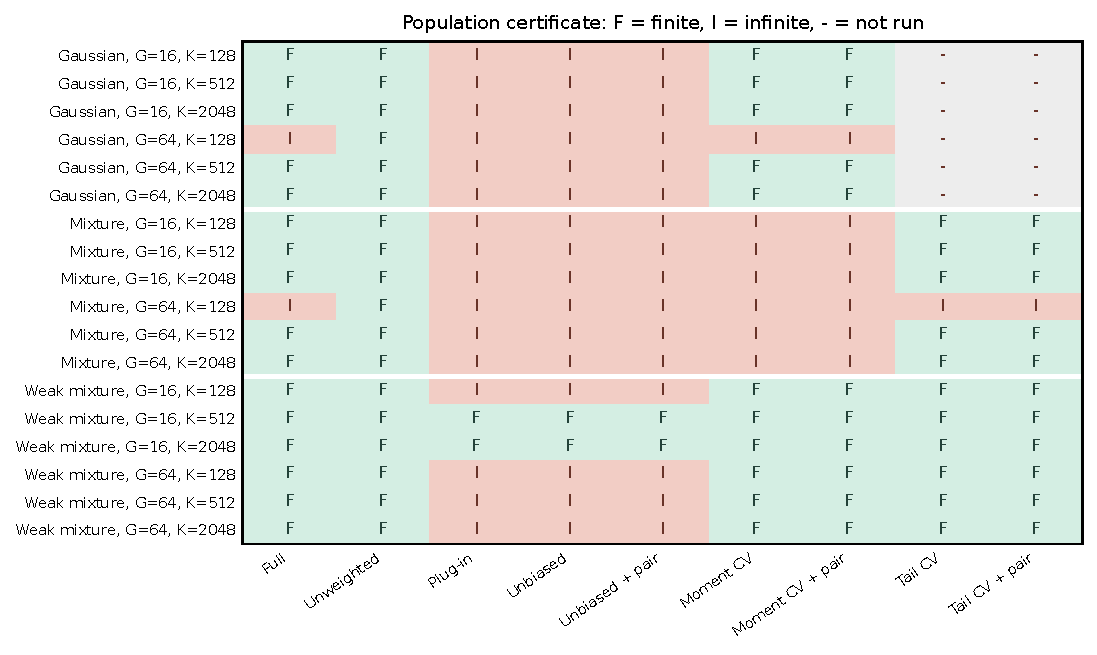
\includegraphics[width=\linewidth]{figures/integrability_grid.pdf}
 \caption{Complete certificate for the executed benchmark methods. The statuses agree for $d=1$ and $d=8$, so the dimensions share a row. Each row therefore represents ten executed cells per method across both dimensions and five seeds. The classification is derived from the population recursion, independently of particle outcomes.}
 \label{fig:complete-certificate}
\end{figure}

\section{Factor families and implementation details}\label{app:protocol}
For indices $g=0,\ldots,G-1$ and $j=0,\ldots,d-1$, set $\theta_{gj}=2\pi(g+0.37j)/G$. Each factor is a product over coordinates. The Gaussian family uses variance $v_{gj}=0.5+0.15\sin\theta_{gj}$ and mean $0.35+0.3\cos\theta_{gj}$. The two-component mixture family uses the same component variance, component means
\[
 0.1\cos\theta_{gj}\ \pm\ (0.7+0.2\cos(2\theta_{gj})),
\]
and positive-component weight $0.5+0.1\sin(\theta_{gj}+0.7)$. The weak mixture family uses
\[
 v_{gj}=\left[1+\frac{4+2\sin\theta_{gj}}G\right]^{-1},\qquad
 \mu_{gj,\pm}=\frac{0.4\cos\theta_{gj}}G
 \pm\frac{0.6+0.1\cos\theta_{gj}}{\sqrt G},
\]
with the same component weights. All component variances are below one, so their residual tail precisions are nonnegative. The Gaussian and ordinary mixture have identical tail certificates despite their different interior geometry.

At each step, weights are multiplied using the left-endpoint potential and states receive the Euler drift and Gaussian noise. Systematic resampling is performed when the effective sample size is below half the particle count. Computation uses double precision, one GPU per task, four allocated CPU cores, and one numerical-library thread. Timing includes sampling, weighting, and resampling, with GPU synchronization at the measured boundaries. Factor reference quadrature and final metric computation are outside the sampler timing. The score-evaluation count records particle--factor evaluations and counts both batches in paired methods.

The raw endpoint sample for each benchmark cell contains all particles and normalized weights. Reference grids, densities, cumulative distribution functions, step metrics, runtime metadata, configuration, and completion records accompany each cell. The one-step study retains weighted histograms and the largest-weight particles, as specified before execution. Independent verification recomputes benchmark metrics using separate SciPy routines and checks all recovered file hashes against the remote manifest.

\section{Matrix-valued bounded tail control}
\label{sec:matrix-tail-extension}

The strict-domain argument extends to Gaussian mixtures with a shared component covariance within each factor. It uses the finite-dimensional Gaussian quadratic integral and a vector density-envelope argument.

Let $x\in\mathbb R^d$. For factor $g$, assume
\[
r_g(x)=-A_gx+d_g+b_g(x),\qquad A_g=A_g^\top,\qquad \|b_g(x)\|\leq B_g.
\]
Let $A_\Sigma=\sum_{g=1}^GA_g$ and define
\[
C=\frac12\left(A_\Sigma^\top A_\Sigma-\sum_{g=1}^GA_g^\top A_g\right),\qquad
L=I-\frac h2\left((1+\kappa)A_\Sigma+\kappa I\right).
\]
Then $C=C^\top$; simultaneous diagonalization of the matrices $A_g$ is not assumed. The bounded terms and vectors $d_g$ contribute at most linearly to the logarithm of the density ratio and do not change the quadratic coefficient.

Assume that the incoming normalized density satisfies the tail envelope
\[
\log p_X(x)=-\frac12x^\top V^{-1}x+O(1+\|x\|),\qquad V\succ0.
\]
The conclusion below concerns this Gaussian covariance envelope for a generally non-Gaussian density. Exact Gaussianity is used only for the auxiliary quadratic calculation that identifies the strict precision condition.

\begin{theorem}[Strict matrix tail certificate]
\label{thm:matrix-tail}
Let $h>0$ and $\kappa>0$. Suppose that the incoming density satisfies the displayed tail envelope, the potential is $x^\top Cx+O(1+\|x\|)$, and the Euler transition is $Y=LX+q(X)+\sqrt{\kappa h}\,\xi$, with $\sup_x\|q(x)\|<\infty$. Set $H=V^{-1}-2hC$. If $H\succ0$, the conditional weighted integral is finite and the propagated normalized density has tail covariance
\[
V^+=LH^{-1}L^\top+\kappa hI\succ0.
\]
If $H$ has a strictly negative eigenvalue, the conditional integral is infinite. The positive-semidefinite boundary is unclassified. On a finite grid, if every batch shares the full-factor matrices $C_k,L_k$, the recursion has the same strict-domain decisions for full-factor and tail-controlled weighting, for every fixed finite batch size.
\end{theorem}

\begin{proof}
The quadratic part of the incoming tail envelope multiplied by the exponential weight is $-x^\top Hx/2$. If $H\succ0$, completing the square in the Gaussian envelope gives a finite reference integral. Its linear image under $L$ has covariance $LH^{-1}L^\top$, and the independent Euler noise has covariance $\kappa hI$. Thus $V^+\succ0$ because $\kappa h>0$, without requiring $L$ to be invertible. The bounded linear remainder in the incoming log density is absorbed into the $O(1+\|x\|)$ envelope.

If $Hv=\lambda v$ with $\lambda<0$, restrict the integral to a fixed bounded tube around the line $x=tv$. The quadratic exponent on that tube contains $-\lambda t^2/2$, which grows strictly quadratically in $|t|$; linear and bounded-remainder terms contribute at most $O(|t|+1)$. The tube integral is infinite.

For the vector density envelope, use the reference joint Gaussian $X\sim\Normal(0,H^{-1})$, $Y=LX+\sqrt{\kappa h}\,\xi$. Write $W=LH^{-1}L^\top+\kappa hI$. Its conditional mean is $\E[X\mid Y=y]=H^{-1}L^\top W^{-1}y$, and its conditional covariance is independent of $y$. A bounded displacement of norm at most $B$ changes the transition-density ratio by factors between
\[
\exp\{-B\|y-Lx\|/(\kappa h)-B^2/(2\kappa h)\}
\quad\text{and}\quad
\exp\{B\|y-Lx\|/(\kappa h)\}.
\]
Combining this with the weighted input envelope gives conditional density-ratio bounds by constants times
\[
\exp\{\pm c_0\pm c_1\|X\|\pm c_2\|y-LX\|\}.
\]
The inequality $\|y-LX\|\leq\|y\|+\|L\|\|X\|$ and Gaussian exponential moments give an upper conditional bound $\exp\{C_1\|y\|+C_2\}$. For the lower bound, Jensen's inequality applied to the positive conditional density ratio gives a lower logarithmic bound because conditional Gaussian first moments of $X$ and $y-LX$ grow at most linearly in $\|y\|$. Multiplication by the Gaussian marginal with covariance $V^+$ yields
\[
\log p_Y(y)=-\frac12y^\top(V^+)^{-1}y+O(1+\|y\|).
\]
The constants are uniform over every fixed finite history set. In the deterministic common-coefficient case, every history therefore has the same strict domain.
\end{proof}

For an exactly Gaussian incoming density and a purely quadratic potential $x^\top Cx+q^\top x+c_0$, the tilted mean and exact normalizing constant are
\[
b=V^{-1}m+hq,\qquad m^+=H^{-1}b,
\]
\[
\log Z=hc_0-\frac12\log\det V-\frac12\log\det H+\frac12b^\top H^{-1}b-\frac12m^\top V^{-1}m.
\]
The subsequent affine propagation maps this tilted mean by the Euler transition. The implementation checks the normalizing constant against independent two-dimensional quadrature for a non-diagonal covariance. The common-coefficient recursion does not require commuting matrices. The scalar extreme-batch reduction for uncontrolled subsampling remains a separate result.

\section{Tail-matched Gaussian path proposals}
\label{sec:gaussian-twist-theorem}

Gaussian backward recursion and change-of-measure weighting are classical components of twisted and controlled SMC \citep{whiteley2014,heng2020}. The result below applies these constructions to the shared quadratic tail of our specified finite-step operator. It establishes existence of all positive weight moments, without asserting a useful numerical variance bound.

\begin{theorem}[Finite-horizon weight moments under tail matching]
\label{thm:gaussian-twist-moments}
Fix $K<\infty$, positive step lengths $\Delta_k$, and a finite set of batch histories with probability law $\mu$. Let $p_0$ be a nondegenerate Gaussian density. For each history $B$, define
\[
 \gamma_B(x_{0:K})=p_0(x_0)\prod_{k=0}^{K-1}
 e^{\Delta_k g_{B,k}(x_k)}q_{B,k}(x_{k+1}\mid x_k).
\]
Assume that, for finite matrices and vectors $L_k,d_k,C_k=C_k^\top,\ell_k,c_k$, and $Q_k\succ0$,
\begin{align*}
 q_{B,k}(\cdot\mid x)&=\Normal(L_kx+d_k+\delta_{B,k}(x),Q_k),\\
 g_{B,k}(x)&=x^\top C_kx+\ell_k^\top x+c_k+v_{B,k}(x),
\end{align*}
where $\sup_{B,x}\|\delta_{B,k}(x)\|<\infty$ and
$|v_{B,k}(x)|\leq a_k+b_k\|x\|$ uniformly in $B$.
Let $\gamma_0$ set $\delta=v=0$. If $0<Z_0=\int\gamma_0<\infty$, its normalized law $\pi_0=\gamma_0/Z_0$ is nondegenerate Gaussian and
\[
 \E_{B\sim\mu,\,X\sim\pi_0} W(B,X)^p<\infty
 \quad\text{for every fixed }p>0,\qquad
 W=Z_0\gamma_B/\gamma_0.
\]
In particular, $\E W=\sum_B\mu(B)\int\gamma_B$ is the normalizer of the specified random-kernel path law. There is no bound uniform in $K$ or in $p$.
\end{theorem}

\begin{proof}
Write $m_k(x)=L_kx+d_k$ and $\delta=\delta_{B,k}(x)$. Equal transition covariances give the exact identity
\[
 \log\frac{q_{B,k}(y\mid x)}{q_{0,k}(y\mid x)}
 =\delta^\top Q_k^{-1}(y-m_k(x))
   -\tfrac12\delta^\top Q_k^{-1}\delta.
\]
Its absolute value is bounded by a finite constant times
$1+\|x\|+\|y\|$. Adding the potential differences over the finite grid gives
$|\log(\gamma_B/\gamma_0)|\leq c_0+c_1\|x_{0:K}\|$ uniformly over histories. The quadratic exponential $\gamma_0$ has positive-definite joint precision whenever its integral is finite: a negative eigenvalue forces quadratic growth, and a zero eigenvalue leaves a nonintegrable affine exponential along its null direction. Hence $\pi_0$ is a nondegenerate Gaussian on $\R^{d(K+1)}$ and has $\E_{\pi_0}e^{t\|X\|}<\infty$ for every finite $t$. Thus
\[
 \E W^p\leq Z_0^p e^{pc_0}\E_{\pi_0}e^{pc_1\|X\|}<\infty.
\]
Finally, change of measure and the finite sum over $B$ give the normalizer identity. Every constant is for a fixed grid.
\end{proof}

For shared-component-covariance mixtures, the full and tail-controlled scores have bounded corrections to their common affine part. Their potential corrections have at most linear growth, including the without-replacement version. They satisfy the primitive assumptions above whenever the strict full-factor matrix certificate holds. Raw subsampling with batch-dependent quadratic coefficients does not satisfy these assumptions.

\paragraph{Backward Gaussian construction.}
Let $g_{0,k}(x)=x^\top C_kx+\ell_k^\top x+c_k$. Define
$\psi_k(x)=\exp(\tfrac12x^\top J_kx+j_k^\top x+a_k)$ with terminal $J_K=0,j_K=0,a_K=0$. For $H_k=Q_k^{-1}-J_{k+1}\succ0$, put
\[
 T_k=Q_k^{-1}H_k^{-1}Q_k^{-1}-Q_k^{-1},\qquad
 \nu_k=Q_k^{-1}H_k^{-1}j_{k+1}.
\]
Completing the square in $e^{\Delta_k g_{0,k}}q_{0,k}\psi_{k+1}$ yields
\begin{align*}
 J_k&=2\Delta_k C_k+L_k^\top T_kL_k,\\
 j_k&=\Delta_k\ell_k+L_k^\top(T_kd_k+\nu_k),\\
 a_k&=\Delta_kc_k+a_{k+1}-\tfrac12\log\det(I-Q_kJ_{k+1})\\
 &\quad+\tfrac12d_k^\top T_kd_k+\nu_k^\top d_k
 +\tfrac12j_{k+1}^\top H_k^{-1}j_{k+1}.
\end{align*}
For $p_0=\Normal(m,V)$, put $P=V^{-1}-J_0$ and $b=V^{-1}m+j_0$. The reference initial law is $\Normal(P^{-1}b,P^{-1})$ and
\[
 \log Z_0=a_0-\tfrac12\log\det V-\tfrac12\log\det P
 +\tfrac12 b^\top P^{-1}b-\tfrac12m^\top V^{-1}m.
\]
The forward conditional reference proposal is
\[
 X_{k+1}\mid X_k=x\sim
 \Normal\bigl(H_k^{-1}[Q_k^{-1}(L_kx+d_k)+j_{k+1}],H_k^{-1}\bigr).
\]
Every $H_k$ and $P$ must be positive definite. These Schur-complement conditions are equivalent to strict positivity of the full Gaussian path precision. The implementation rejects a failing reference. Numerically stable forms $T=J+JH^{-1}J$ and $\nu=j+JH^{-1}j$ avoid subtraction of two large matrices as the step size shrinks.

\paragraph{Independent-path consequence and mixtures.}
For a bounded path observable $f$, independent pairs $(B,X)$ yield consistent self-normalized importance sampling with asymptotic variance $\E[W^2(f-\eta f)^2]/(\E W)^2<\infty$. This follows from the ordinary multivariate central limit theorem and the delta method. It does not establish a resampling-system theorem or guarantee small finite-sample error.

Our optional finite mixture uses reference Gaussian paths with the same joint covariance and different means, with strictly positive fixed mixing probabilities. Relative to any component, its marginal log density differs by a log-sum of affine functions, whose absolute value is at most linear in the path norm. The same argument establishes all positive moments using $W=\gamma_B/\sum_j\omega_j\pi_j$. The sampler evaluates this complete marginal denominator. Weighting by only the selected component would instead be an augmented-component importance construction and must not be confused with this marginal-mixture algorithm or its variance.

\section{Complete oracle and learned benchmark results}\label{app:complete-original-experiments}
The fixed baseline protocol comprises 1,260 main cells and 720 supplementary cells. It uses exact Gaussian and Gaussian-mixture factor scores, isolating random-weight effects from learned-model approximation. Baseline benchmark cells use 8,192 particles, $M=4$, $G\in\{16,64\}$, $d\in\{1,8\}$, $K\in\{128,512,2048\}$, and five random seeds. The reverse-time grid is $u_k=20(1-k/K)^2$, the initial distribution is $\Normal(0,I)$, and $\kappa=1$. The finite-$U$ initialization is an approximation to the exact compositional path. Reference marginals are computed by numerical quadrature on 65,537 points in $[-12,12]$.

The main comparison includes full-factor weighting, an unweighted composed drift, plug-in weighting, unbiased quadratic weighting, a paired cumulant correction, and two moment-matched Gaussian control variants. The supplementary benchmark evaluates tail control and its paired correction on both mixture families. Paired corrections use two independent batches and the positive weight $\exp\{h(\widehat g_1+\widehat g_2)/2-h^2(\widehat g_1-\widehat g_2)^2/8\}$, with the averaged drift; they therefore require twice as many sampled factor evaluations. This correction is an empirical ablation, with no claim of exact exponential unbiasedness.

For the one-step example in \eqref{eq:counterexample}, the supplementary study uses $P\in\{1{,}024,16{,}384,262{,}144,1{,}048{,}576\}$, $M\in\{2,4,8,16,32\}$, and 20 seeds, together with the full-factor update. We retain histograms and the 1,024 largest normalized particle weights for each one-step cell. The benchmark retains complete particle arrays and reference distributions.

All 1,980 baseline cells completed on SCNet RTX 3080 GPUs. We verified the source versions, 13,506 recovered file hashes, all 40 task exit records, and the complete cell configuration lists. Benchmark metrics were recomputed using independent numerical routines. Adaptive quadrature over the real line also verified all 54 reference coordinates, including analytic Gaussian checks. A separately frozen extension adds 1,080 oracle sampling cells and 1,000 learned-density sampling cells, with five complete network trainings (Appendix~\ref{app:extension-protocol}).

\subsection{Local error decreases while the normalizer remains infinite}
Figure~\ref{fig:one-step} shows the one-step experiment. At $P=1{,}048{,}576$, increasing $M$ from 2 to 32 reduces mean potential MSE from $0.46798$ to $0.01857$, approximately a factor of 25. The median ESS fraction rises from $0.000424$ to $0.932706$. Nevertheless, \eqref{eq:counterexample} gives an infinite population normalizer for both batch sizes and every intermediate finite $M$.

For $M=32$, the empirical mean log normalizer is $0.126047$ with standard deviation $0.000259$ across 20 seeds. The full-factor result is $0.122030\pm0.000234$, close to its exact value $0.122049$. No nonintegrable batch was sampled in these 20 runs of $1{,}048{,}576$ particles with $M=32$. The all-strongest event alone has probability $4^{-32}\approx5.42\times10^{-20}$ per batch. Its absence in this finite experiment cannot establish existence of the population target. For $M=2$, the median estimated log normalizer rises from $0.270$ at $P=1{,}024$ to $0.484$ at $P=1{,}048{,}576$, accompanied by severe ESS loss. The proof supplies the divergence result; these finite observations illustrate why it can be visible at small $M$ and inconspicuous at larger $M$.

\begin{figure}[t]
 \centering
 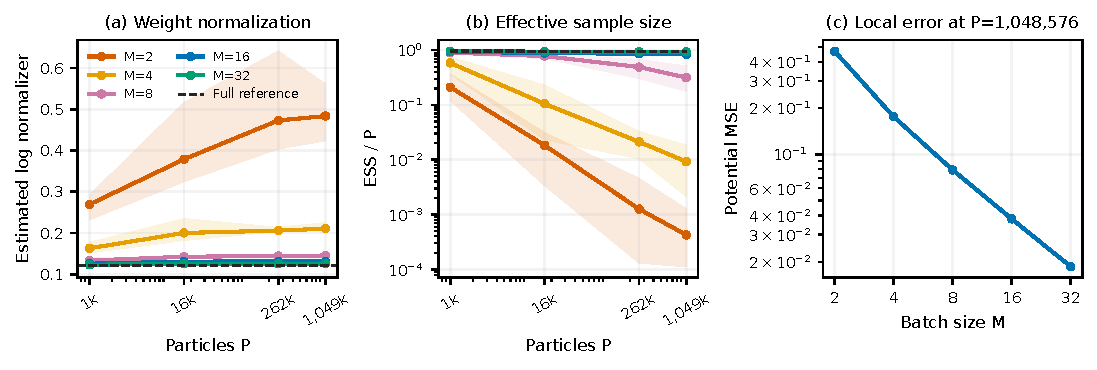
\includegraphics[width=\linewidth]{figures/one_step.pdf}
 \caption{One-step Gaussian counterexample. Panels (a,b) show medians and interquartile ranges over 20 seeds. The dashed reference is the exact full-factor log normalizer in (a) and the empirical full-factor ESS fraction in (b). Panel (c) shows mean potential MSE with one standard deviation at $P=1{,}048{,}576$. Every subsampled curve has an infinite population normalizer.}
 \label{fig:one-step}
\end{figure}

\subsection{Certificates across the benchmark grid}
Appendix Table~\ref{tab:certificates} reports validity over the 12 configurations per family, formed by two group counts, two dimensions, and three time grids. Seeds do not change a certificate. Raw plug-in, unbiased, and paired estimators fail all Gaussian and ordinary-mixture configurations. Moment matching makes the Gaussian estimator exact, but does not certify any ordinary-mixture configuration. Tail matching recovers the full-factor strict domain in both mixture families. The complete configuration-level grid is provided in Appendix~\ref{app:full-results}.

The full-factor discretization also fails for $G=64,K=128$ in the Gaussian and ordinary-mixture families. Its Gaussian denominator first becomes negative at step 100, reaching approximately $-0.003111$. Yet the observed mean marginal W1 is only $0.0141$ in one dimension and $0.0176$ in eight dimensions. Thus a small endpoint sample discrepancy can coexist with an undefined population update even before subsampling. For finite Gaussian configurations, exact weighted-Euler moment recursion separates time error from particle error: at $G=64,K=2048$, the population W1 is approximately $0.000493$, while the eight-dimensional finite-particle mean marginal W1 is $0.0149$.

\subsection{A finite domain does not guarantee accurate or faster inference}
Figure~\ref{fig:accuracy-time} and Table~\ref{tab:matched} compare actual sampler time and endpoint error. For the difficult eight-dimensional ordinary mixture with $G=64,K=512$, all weighted methods have substantial sampling error. Full-factor W1 is $0.881\pm0.372$, tail control is $1.004\pm0.327$, and paired tail control is $1.358\pm0.188$. Their mean total-variation errors over the 256 coordinate-sign patterns are respectively $0.961$, $0.975$, and $0.998$, confirming poor joint-mode coverage. The paired moment control has lower marginal W1, $0.456\pm0.228$, despite an infinite population normalizer. These outcomes demonstrate that finite integrability, marginal accuracy, and joint coverage are distinct properties.

\begin{figure}[t]
 \centering
 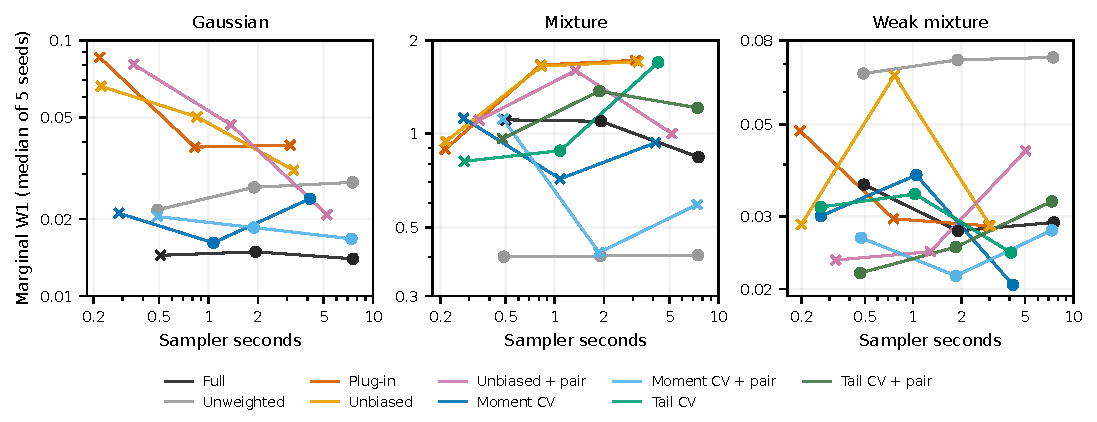
\includegraphics[width=\linewidth]{figures/accuracy_time.pdf}
 \caption{Observed error versus recorded sampler time at $G=64,d=8$, with $K\in\{128,512,2048\}$. Each point is a median over five seeds. Circles denote finite population normalizers and crosses denote infinite ones. Lines connect a method's three time grids and are not fitted performance models.}
 \label{fig:accuracy-time}
\end{figure}

On the weak mixture, paired tail control yields W1 $0.025\pm0.005$, compared with $0.028\pm0.007$ for full weighting, at nearly the same recorded sampler time. Unpaired tail control uses 16 times fewer nonlinear particle--factor evaluations and about $1.86$ times less sampler time, but its W1 rises to $0.043\pm0.026$. We therefore make no general speed--accuracy superiority claim. Gaussian full and exact-control results, complete seed-level metrics, and additional joint diagnostics are retained in the artifacts.

\subsection{Without replacement: batch size changes the finite domain}\label{sec:without-replacement-results}
The prefix/suffix certificate permits an exhaustive scan over batch sizes without enumerating subsets. Table~\ref{tab:batch-thresholds} reports the smallest finite batch size among all $2\le M\le G$ for the benchmark tails. This separate deterministic calculation comprises 936 configurations and agrees with direct subset enumeration in nine smaller cross-checks. The ordinary mixture shares the Gaussian component variances, and dimensions one and eight give identical thresholds here. All larger batch sizes are finite in each displayed case with a finite threshold; this observed ordering is not claimed as a general monotonicity theorem. At $G=64,K=512$, switching from replacement to a uniform subset of size four remains below either family's threshold. Thus removing repeated indices changes the certificate but does not by itself make a small batch valid.

\begin{table}[t]
 \centering
 \caption{Smallest certified finite without-replacement batch size, with $U=20$, $\kappa=1$ and initial variance one. A dash means no finite batch exists, including $M=G$. The mixture rows use the strict tail certificate.}
 \label{tab:batch-thresholds}
 \begin{tabular}{lrccc}
 \toprule
 Tail family & $G$ & $K=128$ & $K=512$ & $K=2048$\\
 \midrule
 Gaussian / ordinary mixture & 16 & 13 & 12 & 12\\
 Gaussian / ordinary mixture & 64 & -- & 60 & 59\\
 Weak mixture & 16 & 3 & 2 & 2\\
 Weak mixture & 64 & 22 & 18 & 17\\
 \bottomrule
 \end{tabular}
\end{table}


\section{Tail-control mechanisms and held-out ablations}\label{app:dual-results}
The five trained mixture networks are unchanged throughout these studies. Nonlinear factor evaluations use analytic mixture scores after a one-time network parameter prediction. Timing consequently measures the reported mixture implementation, rather than repeated evaluation of a large neural score network.

\paragraph{Complete-kernel random correction.}
A separate development study compares interpolation and a positive Poisson correction of a surrogate Euler transition. The conditional identity concerns the complete unnormalized kernel. It does not imply unbiased normalized particle estimates or a resampling variance bound. The configuration is selected on eight learned development targets, then fixed for five networks crossed with ten new datasets. Table~\ref{tab:dual-kernel} reports all 250 confirmation cells. The declared joint requirement is an upper one-sided 95\% bound of $0.002$ on W1 degradation and $0.8$ on the time ratio to the optimized full-factor baseline. None of the approximate methods meets both requirements. The positive-kernel correction has mean W1 difference $0.005139$ with 95\% interval $[-0.000150,0.012475]$ and time ratio $1.0563$. Its observed error interval includes zero; the result establishes no matched-quality speedup.

\begin{table}[ht]
\centering
\caption{Held-out complete-kernel study. Means over five networks crossed with ten datasets, $G=64,d=8,N=32768,K=2048$. Sampling time includes preparation.}
\label{tab:dual-kernel}
\begin{tabular}{lrrrr}
\toprule
Method & Learned W1 & True W1 & Seconds & Joint sign TV\\
\midrule
Full & 0.018273 & 0.019996 & 6.144 & 0.02770\\
Fixed-mean tail & 0.116538 & 0.117157 & 4.342 & 0.09258\\
Interpolation only & 0.019326 & 0.020973 & 3.312 & 0.02987\\
Surrogate, exact correction & 0.020683 & 0.022729 & 15.119 & 0.02949\\
Surrogate, Poisson correction & 0.023412 & 0.025032 & 6.489 & 0.03147\\
\bottomrule
\end{tabular}
\end{table}

\paragraph{Separable strong baseline.}
For a product target, coordinatewise full-factor SMC exploits known independence. Each coordinate is independently resampled at the endpoint, then independently permuted to form joint draws. On the difficult mixture at $N=8192,K=512$, this lowers mean marginal W1 from $0.6973$ to $0.2703$ and joint sign TV from $0.9256$ to $0.3685$. On five learned targets, W1 changes from $0.02514$ to $0.01696$. These are diagnostics on eight distinct parameter sets, with five sampling repetitions on each of three oracle families and five learned datasets. They establish a relevant strong baseline and expose remaining mode loss. Coordinatewise coupling is an existing use of the product structure.

\paragraph{Anchored control.}
On 256 preselected non-anchor state/time points from two trained models and four datasets, exhaustive formula checks and 4096 paired random subsets per point give anchored-to-fixed-mean conditional variance ratios of $0.015397$ for drift and $0.002446$ for potential. The 32 anchor points are reported separately; their zero residual variance follows by construction.

A distinct 150-cell held-out study uses five networks and ten new datasets. Learned-target W1 is $0.016817$ for full weighting, $0.095390$ for fixed-mean tail control, and $0.019673$ for anchored control, all with $N=32768,K=2048,M=4$. The anchored-to-full W1 difference has one-sided 95\% upper bound $0.006076$, exceeding the declared $0.002$ allowance. An algebraically equivalent cache implementation is rerun on the same 50 problems: maximum particle, weight and log-normalizer discrepancies are $1.78\times10^{-15}$, $2.61\times10^{-17}$ and $2.28\times10^{-13}$. Corresponding full, fixed-mean and anchored times are $6.039$, $4.260$ and $3.844$ seconds. The anchored time ratio is $0.63644$ with 95\% interval $[0.63227,0.64048]$. This rerun supplies an implementation comparison on the same cohort, with no additional independent datasets and no change to the failed accuracy criterion.

Post-hoc parameter diagnostics use the saved weighted particles. Full, fixed-mean and anchored posterior-mean MSEs are respectively $0.011167$, $0.027511$ and $0.011664$. Their observed 90\% interval coverages are $88.50\%$, $66.00\%$ and $87.25\%$. These frequencies describe ten data seeds crossed with five trained models; they do not establish population calibration. A separate predeclared development and confirmation study changes the particle, step and batch counts; its results are reported independently.

\paragraph{First and second path moments.}
For a linear Gaussian proposal without intermediate resampling, write the stacked path as $X=m+L\xi$ and its log weight as $X^\top CX+\ell^\top X+c$. Its $p$th weight moment exists exactly when $I-2pL^\top CL$ is positive definite; a nonpositive eigenvalue makes the Gaussian quadratic integral infinite, including the boundary. The exact log moment follows by completing the square. A fixed $G=4,d=3$, 16-step diagnostic on $u\in[1,0]$ has first-moment minimum eigenvalues between $0.36756$ and $0.36796$, and second-moment minimum eigenvalues between $-0.26488$ and $-0.26409$. The normalizer is finite with exact log value $3.615674$, while the unresampled weight lacks a second moment. This statement concerns that path proposal and supplies no variance theorem for a resampled particle system.

\section{Fresh confirmation, nonseparable sensing and proposal development}
\label{app:paper-level-results}

\paragraph{Learned-cohort design.}
The development set crosses training seeds $0,1$ with data seeds $800$--$803$. Nine configurations give 72 cells. The selection rule first requires mean W1 within $0.002$ of the joint full-factor baseline, then chooses the fastest eligible anchored setting. It selects $N=8192,K=1024,M=8$ before confirmation. Five fixed checkpoints crossed with data seeds $900$--$919$ give 100 paired targets. Four settings produce 400 confirmation cells. Every reference, source receipt, dataset regeneration and strict checkpoint reload is independently checked. The independent reference uses 131073 integration nodes. Maximum W1 discrepancies are $1.14\times10^{-6}$ for the learned target and $1.06\times10^{-6}$ for the true target.

The fixed two-way paired bootstrap has 10000 replicates and seed 20260930. The primary gate requires both one-sided 95\% upper bounds: W1 degradation at most $0.002$ and ratio of mean elapsed times below $0.8$. The selected anchor passes against the original joint baseline, with time ratio $0.20341$ and W1 difference $-0.000643$ (two-sided interval $[-0.003037,0.001764]$). It fails against the original coordinatewise baseline, with W1 difference $0.003523$ (interval $[0.001565,0.005545]$). The original-budget anchor $N=32768,K=2048,M=4$ has W1 $0.01988$ in $3.864$ seconds. Time includes method-specific preparation and sample return, but excludes shared references and one-time density-network prediction. These networks do not evaluate neural scores at every diffusion step.

\paragraph{Equal-budget ablation.}
This comparison was added after the original confirmation results were visible. It is explicitly post-hoc. On the same 100 targets, all methods use $N=8192,K=1024$ with the original paired seeds and randomized execution order (seed 20261003). The 100 anchored replays agree with their original saved particles and weights to the recorded numerical tolerance. The two additional baselines and replays give 300 cells, all recovered and independently audited. Sources and raw receipts are checked, all five checkpoints are reloaded, and the same-target reference integrals and same-grid population certificates are reused from the passed parent audit.

The anchored-to-joint ratio of mean times is $0.87967$ with paired 95\% interval $[0.87047,0.89000]$. Its W1 difference is $-0.001681$, interval $[-0.005470,0.001359]$, with one-sided upper bound $0.000924$. Against coordinatewise weighting, the time ratio is $0.82492$, interval $[0.81458,0.83785]$, while the W1 difference is $0.002407$, interval $[0.000250,0.004574]$. Neither comparison passes the inherited joint diagnostic requiring time ratio below $0.8$ and W1 degradation at most $0.002$. The latter reference also violates the accuracy allowance. Figure~\ref{fig:paper-level-diagnostics} separates configuration effects from method effects.

\begin{figure}[h]
\centering
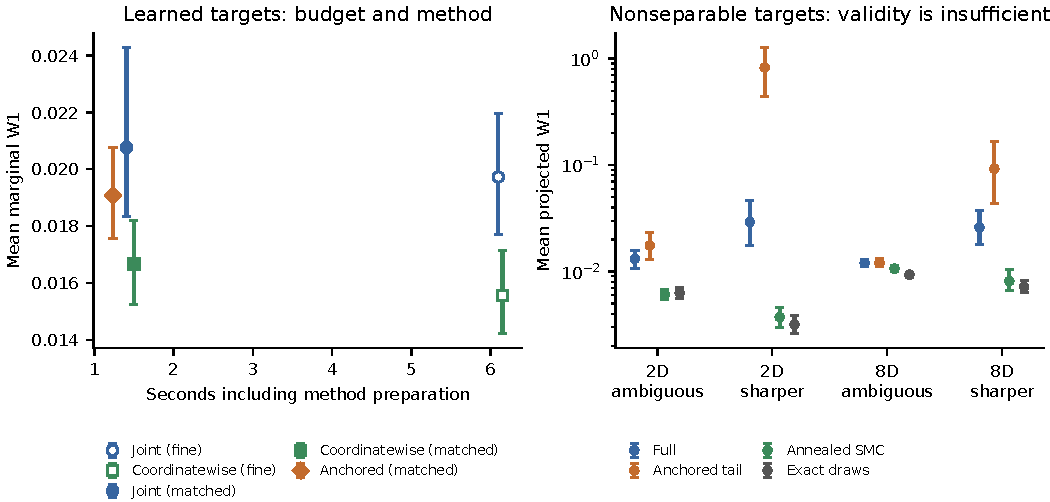
\includegraphics[width=\linewidth]{figures/paper_level_diagnostics.pdf}
\caption{Left: changing the particle/grid budget accounts for most of the original elapsed-time gap. Filled markers use the matched budget; error bars are two-way bootstrap 95\% W1 intervals on the same 100 targets. Right: full and tail-controlled methods share strict integrability certificates, but their nonseparable finite-particle errors differ substantially. Error bars use twenty shared seed clusters.}
\label{fig:paper-level-diagnostics}
\end{figure}

\paragraph{Sensor generator and exact reference.}
Each sensor direction is normalized from a seeded Gaussian vector. In the regular regime, its first two coordinates are replaced by cosine/sine directions on perturbed angles before normalization. Component prior probabilities alternate between $0.65$ and $0.8$. Noise standard deviations lie in $[0.8,0.95]$ for the ambiguous regime and $[0.35,0.43]$ for the regular regime. The latter label denotes sharper observations; sign ambiguity remains. Given one observation, component means are $\pm y_ga_g/(\sigma_g^2+\|a_g\|^2)$ and covariance is $I-a_ga_g^\top/(\sigma_g^2+\|a_g\|^2)$. Enumeration of all signs yields an exact Gaussian mixture, with a common component covariance and exact mixture moments. The independent auditor also computes evidence in observation space and compares the resulting direct likelihood density with this latent-space mixture.

Development seeds $1100,1101$ crossed with both dimensions and regimes yield eight targets and 96 cells. Anchored control fails its development accuracy screen; the predefined least-error fallback selects $N=16384,K=2048,M=8$, with the failure flag retained. The likelihood baseline selects 64 annealing stages, three pCN moves per stage with scale $0.15$, and one global sign-flip Metropolis move. Confirmation seeds $1200$--$1219$ give 80 targets and six methods, for 480 cells. The bootstrap resamples the same data-seed index across dimensions, regimes and methods, for 10000 replicates with seed 20261001.

\begin{table}[h]
\centering\small
\caption{Mean projected W1 by nonseparable setting; twenty seeds in each column.}
\begin{tabular}{lrrrr}
\toprule
Method & $d=2$, ambiguous & $d=2$, regular & $d=8$, ambiguous & $d=8$, regular\\
\midrule
Full & 0.01318 & 0.02917 & 0.01207 & 0.02603\\
Raw batch & 0.01192 & 0.05998 & 0.01236 & 0.02882\\
Fixed tail & 0.02257 & 1.02687 & 0.01409 & 0.51651\\
Anchored tail & 0.01757 & 0.82317 & 0.01203 & 0.09216\\
Annealed SMC & 0.00612 & 0.00373 & 0.01064 & 0.00811\\
Exact draws & 0.00631 & 0.00317 & 0.00934 & 0.00717\\
\bottomrule
\end{tabular}
\end{table}

The independent sensor audit covers all 88 reference assets and all 576 development/confirmation cells. It checks raw sample metrics, exact density and moment calculations, matrix certificates, checksums, configurations and completion markers. Seeded reference samples are reproduced in their original numerical environment. Cross-platform singular-value decompositions can rotate or change signs of Gaussian sampling factors; the local cross-platform report retains the resulting samplewise replay mismatches while all independently recomputed posterior densities, moments and cell metrics agree. Timing is excluded from confirmatory inference because an unrelated training process overlapped the final sampling interval. Raw-batch full-history matrix integrability remains explicitly unclassified.

\paragraph{Gaussian path pilot.}
New seeds $1300,1301$ crossed with both sensor dimensions and regimes give eight development targets. Seven configurations give 56 cells. The proposal uses exact Gaussian backward recursion, independent paths without intermediate resampling, and full path likelihood-ratio correction; a two-component variant uses the complete mixture-density denominator. All full-target proposals share the same specified full Euler target at a given grid. The batch-eight variant targets its own random kernel. Source code, exact references, all final metrics and log-weight normalization are independently audited. Eleven implementation tests pass on the H20, including dense-path Gaussian agreement and nonlinear complete-path density identities.

\begin{table}[h]
\centering\small
\caption{Gaussian path development only. The stopping rule admits no candidate for confirmation. Different particle/grid budgets are shown explicitly.}
\begin{tabular}{lrrrr}
\toprule
Proposal/target & $N$ & $K$ & Projected W1 & Seconds\\
\midrule
Mean Gaussian/full & 8192 & 1024 & 0.22192 & 1.051\\
Anchor Gaussian/full & 8192 & 1024 & 0.26545 & 1.047\\
Two Gaussians/full & 8192 & 1024 & 0.12567 & 1.182\\
Two Gaussians/full & 16384 & 2048 & 0.14606 & 3.012\\
Two Gaussians/batch-eight & 8192 & 1024 & 0.34275 & 1.567\\
Original full weighting & 16384 & 2048 & 0.02500 & 1.633\\
Annealed SMC & 16384 & 64 stages & 0.00702 & 0.106\\
\bottomrule
\end{tabular}
\end{table}

\section{Additional negative development studies}\label{app:continued-iteration}

These studies ask whether tail information provides a useful reference for static posterior sampling after the negative Gaussian-path pilot. Their targets differ from the finite-grid Feynman--Kac path law in Theorem~\ref{thm:gaussian-twist-moments}. We use standard geometric-bridge SMC and Gaussian-reference pCN \citep{delmoral2006,cotter2013}. Gaussian-mixture pCN and SMC have direct prior work \citep{lu2025}; combining these components is not claimed as a methodological first. Both studies fixed their finite configuration lists, development seeds and stopping rules before execution. Neither passed its joint development gate, so neither opened a new performance-confirmation cohort.

\subsection{Tail-informed static bridges on the sensor task}

Let $\widetilde p$ denote the normalized prior times normalized sensor likelihoods. A reference $q$ gives the bridge $\gamma_\beta=q^{1-\beta}\widetilde p^\beta$, $0\leq\beta\leq1$. Its incremental weight is $\exp\{\Delta\beta(\log\widetilde p-\log q)\}$. Reference covariances are $c\Lambda^{-1}$, where $\Lambda=I+\sum_ga_ga_g^\top/\sigma_g^2$ and $c\in\{1,4\}$. The reference uses one, two or four candidate centers from 32 fixed latent-sign EM iterations. Centers and weights are determined only by the available likelihood and observations; no exact posterior or reference sample enters the sampler. Normalized target heights set the reference mixture weights.

At each move, component $j$ is drawn with its reference responsibility at the current point, followed by a pCN move reversible with respect to that component. The resulting mixture kernel is $q$-reversible. Its Metropolis acceptance uses the complete residual $\beta(\log\widetilde p-\log q)$. Every stage also includes a sign-flip proposal with the complete bridge-density ratio. Adaptive temperatures target ESS fraction $0.8$; all nonfinal stages resample, while final weights are retained through the invariant moves. Adaptation does not establish a finite-particle unbiased normalizer estimate.

The twelve candidates cross the three reference choices, two covariance scales and pCN scales $0.5,1$. Three adaptive-prior controls use scales $0.15,0.35,0.65$. Nine fixed-stage prior-SMC controls cross these scales with 32, 64 and 128 temperatures. Full and anchored diffusion are diagnostics. All 26 settings use $N=16384$. Four fresh data seeds, $1400$--$1403$, cross the two dimensions and noise regimes, yielding sixteen targets and 416 cells. These are four shared seed clusters, not 416 independent problems. GPU process snapshots record the same sole process before and after every cell; they are not continuous isolation measurements.

The baseline is the fastest control within $0.001$ of the best control's mean projected W1. A candidate must be at most $0.002$ worse overall, at most $0.004$ worse in every dimension/noise stratum, and below $80\%$ of the mean time of both that baseline and the original 64-stage control. The selected control uses 32 stages and scale $0.35$. No candidate passes. Table~\ref{tab:static-bridge-development} displays the smallest-error candidate descriptively, without promoting it to confirmation.

\begin{table}[h]
\centering\small
\caption{Sensor development only: equal particle counts on sixteen targets. Time includes reference preparation, mode search and returned output. Factor-call counts follow the recorded runner conventions and exclude reference evaluation.}
\label{tab:static-bridge-development}
\begin{tabular}{lrrr}
\toprule
Method & Projected W1 & Seconds & Factor calls ($10^6$)\\
\midrule
Retuned prior-SMC, 32 stages & 0.006626 & 0.06898 & 25.362\\
Original prior-SMC, 64 stages & 0.007051 & 0.13393 & 50.528\\
Best-error tail mixture, $c=4$ & 0.010256 & 0.06110 & 3.354\\
Full diffusion, 2048 steps & 0.018110 & 1.91124 & 402.653\\
Anchored diffusion, 2048 steps & 0.318881 & 3.69364 & 268.435\\
\bottomrule
\end{tabular}
\end{table}

The smallest-error candidate reduces recorded factor calls by $86.8\%$ but elapsed time by only $11.4\%$ against the retuned control. Its W1 difference is $0.003629$, beyond the $0.002$ allowance. The eight-dimensional regular stratum contributes most of this discrepancy: W1 is $0.02209$ versus $0.00756$, including one candidate run at $0.06725$. The other three candidate-stratum means lie between $0.00282$ and $0.00877$. These observations motivate separate checks of reference coverage and implementation overhead; they do not identify a unique causal failure mechanism.

The independent audit passes all sixteen exact-reference assets and all 416 cells. It recomputes nine metrics per cell, checks observation-space evidence against the latent mixture, reproduces the seeded references in the original environment, verifies source and file hashes, and checks bridge temperatures, weight normalization, incremental log normalizers and evaluation counts. The frozen legacy samplers do not retain incremental log-normalizer records, so that particular check is unavailable for them. A numerical audit does not turn the failed performance screen into a successful result.

For this static sensor task, the likelihood is bounded. Consequently prior-reference importance weights already have every positive moment. Tail matching here cannot be interpreted as repairing missing static importance-weight moments. Its practical value would require separate finite-budget accuracy or cost evidence.

\subsection{Composition of independently trained factor models}

We assign the five previously trained checkpoints to five nonorthogonal unit directions in $\R^2$. With $\theta\sim\Normal(0,I_2)$, observations satisfy $y_g=a_g^\top\theta+s_go_g+\sigma_g\epsilon_g$, with equiprobable signs and independent standard Gaussian noise. Direction angles are $(g+1/4)\pi/5$, noise scales are $0.55+0.10g$ and offsets are $0.40+0.15g$, for $g=0,\ldots,4$. Each checkpoint supplies a two-component scalar posterior $\widehat f_g$. The sampler receives only its frozen mixture parameters, defining the prior-corrected target
\[
 \widetilde p_{\mathrm{learned}}(\theta)=\varphi_2(\theta)
 \prod_{g=0}^4\frac{\widehat f_g(a_g^\top\theta)}{\varphi_1(a_g^\top\theta)}.
\]
For each unit direction, $\varphi_2(\theta)\widehat f_g(a_g^\top\theta)/\varphi_1(a_g^\top\theta)$ integrates to one; the scalar factor alone is not a normalized density on $\R^2$. The common component precision is $\Lambda=I+\sum_g(v_g^{-1}-1)a_ga_g^\top\succ0$. Enumeration of 32 components supplies the normalized evaluation density. The small factor count also makes enumeration a legitimate competing algorithm, whose preparation and sampling costs are included below. The analytic generating model is used separately to measure learned-target error. Thus the interface is checkpoint-only, but the experiment is still synthetic and analytically tractable.

All methods use $N=4096$. References use sixteen fixed prior starts and fifty latent-component EM iterations, with at most four distinct centers. Three prior-SMC scales, $0.15,0.35,0.65$, receive the same development data. Remaining settings are a single Gaussian, the mixture candidate, direct IS from that mixture, mixture SMC with $10\%$ independent full-reference refreshes, and exact enumeration. Three paired sampler repeats cross four new data seeds, $1600$--$1603$, producing 96 cells. The five heads form one fixed bank, not five training repetitions of this experiment.

The primary candidate is fixed as mixture SMC. Its comparator is the fastest prior-SMC setting within $0.001$ of the best prior-SMC error, here scale $0.65$. The expansion rule again requires mean W1 degradation at most $0.002$ and total-time ratio below $0.8$. The observed difference is $0.000657$, but the ratio is $0.8410$; confirmation therefore remains closed. Diagnostic settings cannot replace the primary candidate after observing these data.

\begin{table}[h]
\centering\small
\caption{Checkpoint-only development: four data problems and three paired sampler repeats, with one fixed factor bank. W1 uses the analytic Gaussian-mixture CDF. Total time includes the same measured neural-prediction cost for each method; sampling time includes method-specific reference construction.}
\label{tab:learned-factor-development}
\begin{tabular}{lrrr}
\toprule
Method & Projected W1 & Sampling seconds & Total seconds\\
\midrule
Prior-SMC, scale $0.15$ & 0.012943 & 0.06150 & 0.11932\\
Prior-SMC, scale $0.35$ & 0.009714 & 0.06687 & 0.12468\\
Prior-SMC, scale $0.65$ & 0.010056 & 0.06114 & 0.11895\\
Single-Gaussian SMC & 0.010713 & 0.02869 & 0.08650\\
Mixture SMC (primary) & 0.010713 & 0.04223 & 0.10004\\
Mixture direct IS & 0.012924 & 0.01178 & 0.06959\\
Mixture with global refresh & 0.010865 & 0.02898 & 0.08679\\
Exact enumeration & 0.011157 & 0.00595 & 0.06376\\
\bottomrule
\end{tabular}
\end{table}

The reference search retains only one distinct center on each of these four problems. The paired single-Gaussian and mixture outputs consequently agree, so this cohort does not demonstrate a multimodal benefit. Their measured preparation and runtime differences are reported without attributing them to a distinct sampling distribution. The first problem's five neural predictions take $0.22759$ seconds; each of the other three takes about $0.00122$ seconds. The shared mean contribution is $0.05781$ seconds per query. Cold-start cost is retained under the frozen rule; sampling-only and steady-state-serving interpretations are distinct, post-hoc cost questions.

Projected W1 between the learned and generating posteriors ranges from $0.00382$ to $0.01090$. This model error is separate from sampler error against the learned target. The empirical-versus-learned W1 integral uses Gaussian-CDF primitives and interval root finding, avoiding a random reference-sample floor; root-location error and floating-point roundoff remain distinct.

An independent audit passes all four learned/true reference pairs and all 96 cells. It checks direct prior-corrected product densities and two-dimensional numerical normalization, then recomputes sample moments and 32 projected W1 values using separate 32769-node Gaussian-CDF quantizations. The W1 check uses a half-grid-spacing and analytic tail bound, with a $10^{-9}$ numerical allowance that is not a certified floating-point bound. File/source receipts, frozen selection, payload hashes and single-process GPU snapshots are also checked. The learned-versus-generating model-error quadrature is not independently recomputed by this auditor.

Exact enumeration is faster on this small task. The results establish a tested composition interface and a negative development screen, not high-dimensional scaling, a general efficiency advantage or an external application result.

\section{Additional baseline comparisons}\label{app:baseline-tables}
These tables retain the complete method comparisons summarized in Section~\ref{sec:experiments}.

\begin{table}[ht]
 \centering
 \caption{Number of configurations with finite population normalizers, out of 12 per family. A dash denotes an unrun method; tail matching coincides with the Gaussian control on Gaussian factors. Unweighted updates are Markov kernels with unit weights, so finiteness alone is immediate and does not establish target accuracy.}
 \label{tab:certificates}
 \begin{tabular}{lccc}
 \toprule
 Method & Gaussian & Mixture & Weak mixture\\
 \midrule
 Full & 10/12 & 10/12 & 12/12\\
 Unweighted & 12/12 & 12/12 & 12/12\\
 Plug-in & 0/12 & 0/12 & 4/12\\
 Unbiased & 0/12 & 0/12 & 4/12\\
 Unbiased + pair & 0/12 & 0/12 & 4/12\\
 Moment CV & 10/12 & 0/12 & 12/12\\
 Moment CV + pair & 10/12 & 0/12 & 12/12\\
 Tail CV & -- & 10/12 & 12/12\\
 Tail CV + pair & -- & 10/12 & 12/12\\
 \bottomrule
 \end{tabular}
\end{table}

\begin{table}[ht]
 \centering
 \caption{Matched configuration $G=64,d=8,K=512$. W1 is mean $\pm$ one standard deviation over five seeds; seconds are medians. A superscript $\infty$ marks an infinite population normalizer. All methods use 8,192 particles.}
 \label{tab:matched}
 \begin{tabular}{lrrrr}
 \toprule
 & \multicolumn{2}{c}{Mixture} & \multicolumn{2}{c}{Weak mixture}\\
 Method & W1 & Seconds & W1 & Seconds\\
 \midrule
 Full & $0.881\pm0.372$ & 1.921 & $0.028\pm0.007$ & 1.909\\
 Unweighted & $0.404\pm0.003$ & 1.897 & $0.072\pm0.001$ & 1.896\\
 Plug-in & $1.662\pm0.021^{\infty}$ & 0.822 & $0.053\pm0.051^{\infty}$ & 0.754\\
 Unbiased & $1.649\pm0.010^{\infty}$ & 0.828 & $0.070\pm0.038^{\infty}$ & 0.764\\
 Unbiased + pair & $1.608\pm0.099^{\infty}$ & 1.341 & $0.032\pm0.014^{\infty}$ & 1.282\\
 Moment CV & $0.742\pm0.097^{\infty}$ & 1.077 & $0.052\pm0.040$ & 1.047\\
 Moment CV + pair & $0.456\pm0.228^{\infty}$ & 1.865 & $0.022\pm0.005$ & 1.850\\
 Tail CV & $1.004\pm0.327$ & 1.081 & $0.043\pm0.026$ & 1.027\\
 Tail CV + pair & $1.358\pm0.188$ & 1.876 & $0.025\pm0.005$ & 1.847\\
 \bottomrule
 \end{tabular}
\end{table}

\section{Extended sampling and learned-posterior protocols}\label{app:extension-protocol}
The extension protocol is frozen separately from the 1,980-cell baseline. Its oracle matrix contains 1,080 unique sampling cells. For each of the three factor families, it uses $G=64$, $d\in\{1,8\}$, $K\in\{512,2048\}$, five seeds, $P=8192$ and $U=20$. The methods are full weighting, unbiased weighting with and without replacement, and tail control with and without replacement. Each subsampled method uses $M\in\{2,4,8\}$; the full baseline is shared across batch sizes. This gives 780 cells. At $G=64,d=8,K=512,M=4$, the sensitivity study adds $P\in\{32768,131072\}$ at $U=20$ and $U\in\{10,30\}$ at $P=8192$ for every family, method and seed, adding 300 cells. Varying $U$ with $K$ fixed changes both initialization and the time grid, so this comparison does not isolate initialization error alone.

Without-replacement batches use independent double-precision uniform random keys for all $G$ factors and select the $M$ smallest keys. The resulting subset is uniform under the ideal continuous-key law. Selection requires $O(PG)$ work and is included in recorded sampler time. The displayed particle--factor evaluation count measures the selected scores and does not imply that subset selection is independent of $G$.

\subsection{Conditional density learning}
We use mixture density networks \citep{bishop1994} in a controlled neural-posterior setting; conditional density learning from simulator samples is established in simulation-based inference \citep{papamakarios2016}. The simulator is
\[
 \theta\sim\Normal(0,1),\quad Z\sim\operatorname{Uniform}\{-1,+1\},\quad
 y=\theta+Zb+\sigma\epsilon,\quad \epsilon\sim\Normal(0,1).
\]
During training, $\sigma\sim\operatorname{Uniform}[0.45,1.2]$ and $b\sim\operatorname{Uniform}[0.3,1.3]$. A network with three hidden layers of width 128 and SiLU activations maps $(y/3,\log\sigma,b)$ to four outputs. These parameterize two component means as center plus or minus a softplus separation, one common variance as $0.02+0.96\operatorname{sigmoid}(v)$, and two positive mixture weights using one logit. The variance restriction gives nonnegative residual tail precisions for the certificate. It is an architectural assumption, not an estimated property of a general score network.

Five independent training seeds each use 40,000 Adam updates with batches of 2,048 fresh joint simulator samples, giving 81,920,000 training pairs per seed. The learning rate decreases from $3\times10^{-4}$ to $3\times10^{-5}$ by a cosine schedule. Training minimizes conditional negative log likelihood and receives no exact posterior or score labels. We use the fixed final checkpoint for every seed. Validation on 100,000 fixed heldout pairs is recorded every 2,000 updates; it does not select checkpoints. Initial and final weights, loss histories and final checkpoint hashes are retained. A separate local audit evaluates the saved final networks on 100,000 newly generated heldout pairs and compares their negative log likelihood with the exact posterior value on those same pairs.

The exact conditional posterior, used only for evaluation, has common variance $v=\sigma^2/(1+\sigma^2)$, means $(y-b)/(1+\sigma^2)$ and $(y+b)/(1+\sigma^2)$, and weights proportional to
\[
 \exp\!\left(-\frac{(y-b)^2}{2(1+\sigma^2)}\right),\qquad
 \exp\!\left(-\frac{(y+b)^2}{2(1+\sigma^2)}\right).
\]
An independent likelihood-times-prior calculation checks this identity. The learned factors are mixtures with a closed-form Ornstein--Uhlenbeck convolution, so their evolving scores and tail variances are available exactly conditional on the trained network. The experiment therefore tests learned conditional densities with known tail structure, and does not certify arbitrary neural score models.

\subsection{Grouped datasets and error decomposition}
For each of five dataset seeds, $G\in\{16,64\}$ and $d\in\{1,8\}$, generate one shared $\theta_j\sim\Normal(0,1)$ per coordinate and $G$ conditionally independent observations. With $\alpha_{gj}=2\pi(g+0.37j)/G$, use
\[
 \sigma_{gj}=0.45+0.75(0.5+0.5\sin\alpha_{gj}),\qquad
 b_{gj}=0.8+0.5\cos(2\alpha_{gj}).
\]
Each observation has an independent sign and Gaussian noise. The same dataset and learned factor parameters are used by all five sampling methods. Every checkpoint/dataset pair is evaluated at $K\in\{512,2048\}$ with $P=32768$, $M=4$, $U=20$, $\kappa=1$, standard Gaussian initialization, and the baseline resampling rule. This gives 1,000 sampling cells, across five training seeds, five dataset seeds, four $(G,d)$ configurations, two grids and five methods.

We distinguish particle W1 against the normalized composition of learned factors, particle W1 against the true posterior composition, and the W1/KL discrepancy between the true and learned compositions. The two particle errors do not add to an exact decomposition of W1. Means and standard deviations across the 25 crossed checkpoint/dataset pairs describe dispersion; those pairs are not 25 independent training runs. The main figure uses the preselected finer grid, with the coarser grid retained in the appendix and complete tables. Network parameters are predicted once per context, before particle sampling. Setup time is recorded separately, and these timings do not measure repeated neural-network evaluations at evolving particle states.

\subsection{Independent verification of the trained densities}
All five networks contain 34,052 parameters and complete the prescribed 40,000 updates. Their initial and final checkpoints have finite weights and distinct hashes, with parameter-change Euclidean norms between 7.48 and 7.79. Table~\ref{tab:training-verification} reports every training seed. The independent conditional KL uses 1,024 new contexts and 16,385 quadrature points on $[-16,16]$; both component-mixture densities integrate to one within the audit tolerance. The original GPU KL diagnostics use different heldout contexts and are retained separately.

\begin{table}[ht]
 \centering
 \caption{Fixed final checkpoints. Validation NLL uses the original 100,000-pair GPU validation set. Independent KL is $\E_c[\operatorname{KL}(p(\theta\mid c)\|q_\psi(\theta\mid c))]$ averaged over 1,024 new contexts, with the displayed value multiplied by $10^5$. Every row is independently checked.}
 \label{tab:training-verification}
 \begin{tabular}{rrr}
 \toprule
 Training seed & Recorded validation NLL & Independent KL $\times10^5$\\
 \midrule
 0 & 1.091306 & 6.477\\
 1 & 1.091242 & 4.828\\
 2 & 1.091280 & 8.880\\
 3 & 1.091315 & 9.242\\
 4 & 1.091384 & 12.994\\
 \bottomrule
 \end{tabular}
\end{table}

A separate 100,000-pair Monte Carlo comparison evaluates learned and exact-posterior negative log likelihood on the same fresh samples. Its excess-NLL estimates range from $-2.38\times10^{-5}$ to $1.72\times10^{-4}$, with standard errors between $3.29\times10^{-5}$ and $5.13\times10^{-5}$. A negative finite-sample estimate is compatible with Monte Carlo noise; it is not a negative KL divergence. The integrated conditional KL and the composed-density errors supply separate distribution-level diagnostics.

\section{Complete extended sampling results}\label{app:extension-results}
Figure~\ref{fig:extension-sampling} includes every oracle sampling configuration at $P=8192,U=20$. Across the full 1,080-cell oracle extension, all 600 full-factor or tail-controlled cells have finite normalizers; all 480 raw unbiased cells have infinite normalizers. In particular, $M\in\{2,4,8\}$ remains below the finite thresholds at $G=64$ for these tails. The statement is a certificate calculation, not an inference from observed particle errors.

\begin{figure}[p]
 \centering
 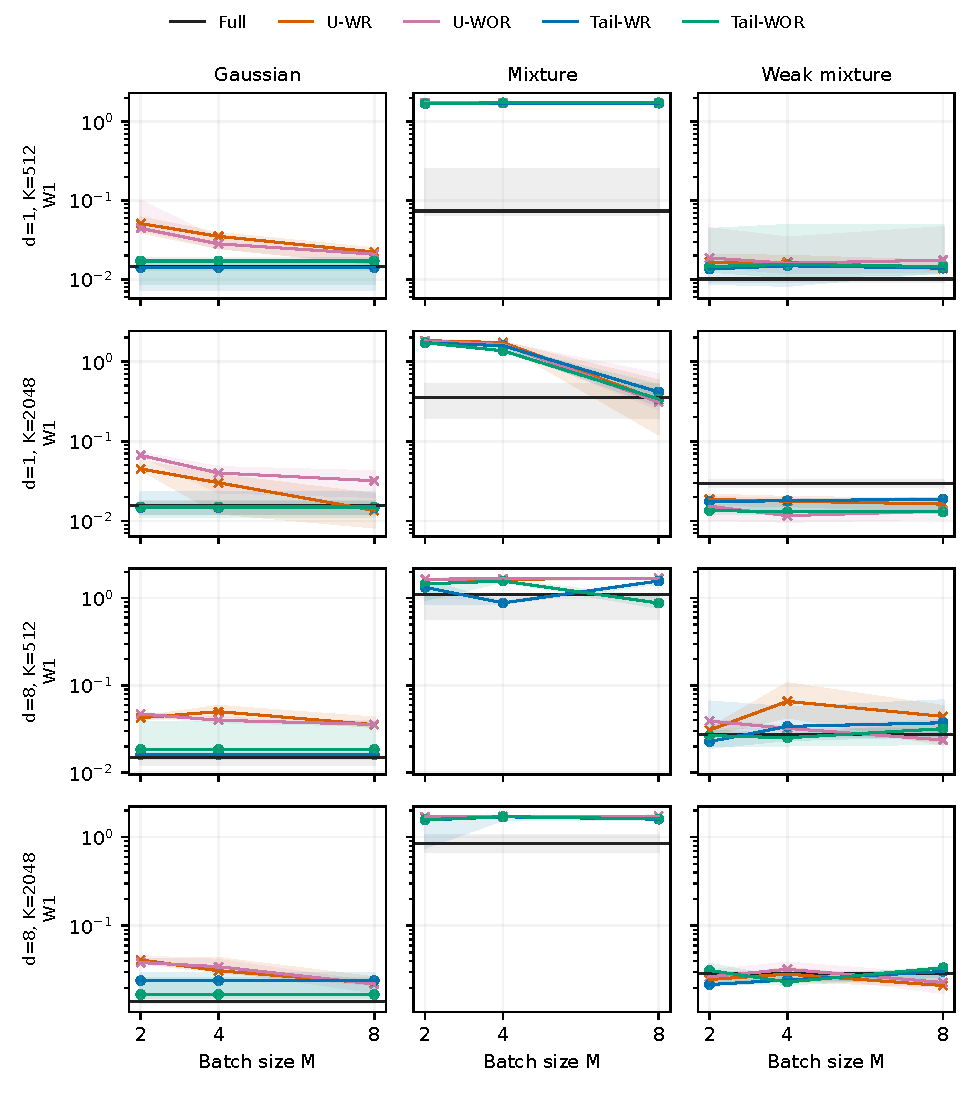
\includegraphics[width=\linewidth]{figures/extension_sampling.pdf}
 \caption{Complete oracle batch-size comparison. Curves show median marginal W1 and interquartile ranges across five seeds. The horizontal black line and band show the full-factor median and interquartile range. Circles denote finite normalizers and crosses infinite ones. Every row uses $G=64,P=8192,U=20$; its dimension and grid size are labeled at left. All four subsampled methods and all three batch sizes are shown.}
 \label{fig:extension-sampling}
\end{figure}

\subsection{Particle count and terminal-noise sensitivity}
Figure~\ref{fig:extension-sensitivity} reports the full sweep at $G=64,d=8,K=512,M=4$. Increasing particles does not guarantee monotone improvement over this range. For the ordinary mixture, full-factor mean W1 decreases from $0.881$ at $P=8192$ to $0.650$ at $P=131072$, while tail control without replacement remains poor, with mean W1 $1.440$ and $1.470$ respectively. For the weak mixture, raw with-replacement weighting improves from $0.0704$ to $0.0098$ while remaining nonintegrable, whereas finite tail control without replacement has mean W1 $0.0250$, $0.0194$ and $0.0357$ across the three particle counts. Thus increasing particles does not repair a failed population certificate, and the observed finite methods need not improve monotonically.

Changing $U$ from 10 through 20 to 30 at fixed $K$ leaves the full-factor and tail-control certificates finite and the raw certificates infinite in every tested cell. Full-factor mean W1 is $0.0265$, $0.0280$ and $0.0282$ for the weak mixture, and $0.801$, $0.881$ and $0.711$ for the ordinary mixture. Because this intervention changes the entire time grid as well as the initialization level, these data cannot identify an initialization-only effect.

\begin{figure}[p]
 \centering
 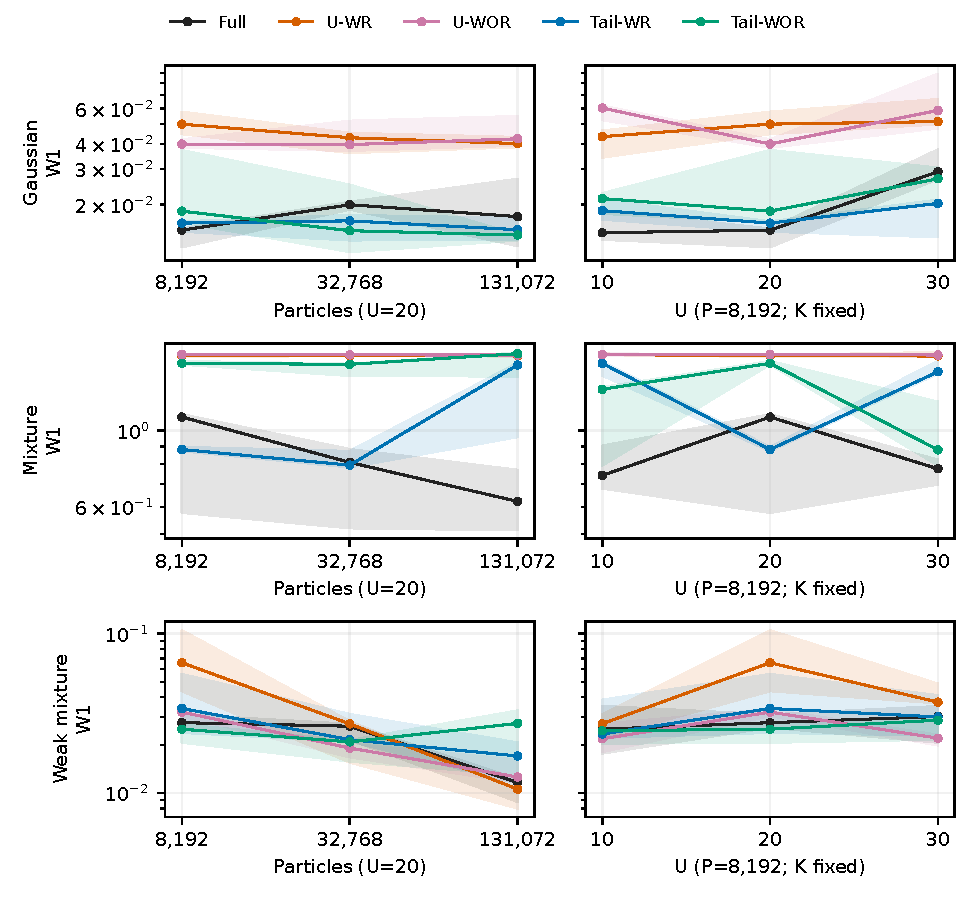
\includegraphics[width=\linewidth]{figures/extension_sensitivity.pdf}
 \caption{Complete particle-count and terminal-noise sweeps, with median marginal W1 and interquartile ranges across five seeds. Here circles mark every measured setting and do not encode validity: Full, Tail-WR and Tail-WOR are finite throughout; U-WR and U-WOR are infinite throughout. Left panels vary $P$ at $U=20$; right panels vary $U$ at $P=8192$. Both hold $K=512$ fixed.}
 \label{fig:extension-sensitivity}
\end{figure}

\subsection{Coarser learned-posterior grid}
Figure~\ref{fig:learned-coarse} retains all 25 pairs at $K=512$. Both grids have the same certificate classifications, while endpoint errors depend on the grid. Tables~\ref{tab:learned-512} and~\ref{tab:learned-2048} report all configuration means and standard deviations; the released CSVs contain every individual cell, KS and moment diagnostics, prediction time and sampler time. The 100 distinct learned compositions are also retained individually.

\begin{figure}[htbp]
 \centering
 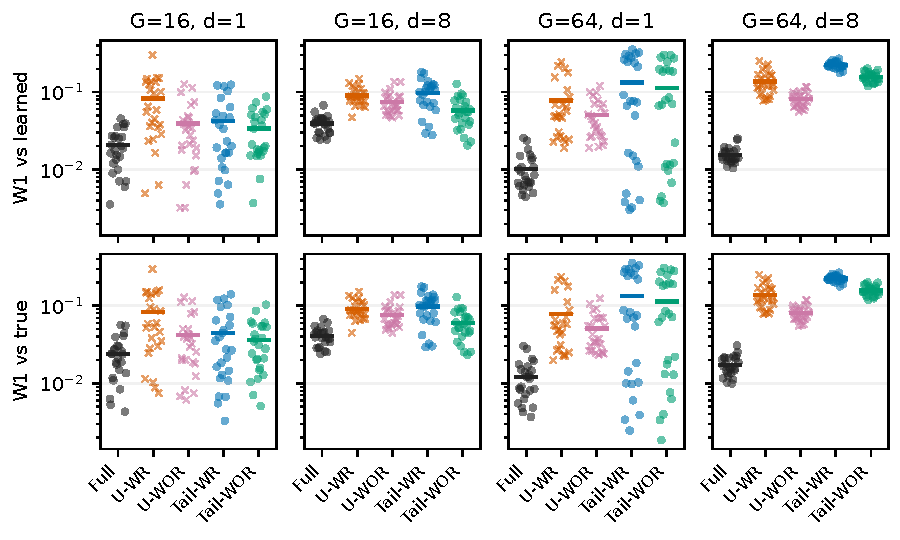
\includegraphics[width=\linewidth]{figures/learned_results_coarse.pdf}
 \caption{Complete learned-posterior comparison at $K=512$, using the same display and validity conventions as Figure~\ref{fig:learned}. All training and dataset seeds are included.}
 \label{fig:learned-coarse}
\end{figure}
\begin{table}[htbp]
 \centering
 \caption{Complete learned-posterior results at $K=512$. W1 values are means $\pm$ sample standard deviations across 25 crossed checkpoint/dataset pairs. Time is mean recorded sampler seconds. F and I denote finite and infinite population normalizers.}
 \label{tab:learned-512}
 \small
 \begin{tabular}{rrlcllr}
 \toprule
 $G$ & $d$ & Method & Domain & W1 vs learned & W1 vs true & Seconds\\
 \midrule

16 & 1 & Full & F & $0.0207\pm0.0116$ & $0.0240\pm0.0144$ & 0.59\\
16 & 1 & U-WR & I & $0.0828\pm0.0679$ & $0.0824\pm0.0690$ & 0.76\\
16 & 1 & U-WOR & I & $0.0392\pm0.0336$ & $0.0417\pm0.0350$ & 0.73\\
16 & 1 & Tail-WR & F & $0.0420\pm0.0391$ & $0.0450\pm0.0415$ & 0.99\\
16 & 1 & Tail-WOR & F & $0.0339\pm0.0223$ & $0.0364\pm0.0253$ & 1.00\\
\midrule
16 & 8 & Full & F & $0.0392\pm0.0103$ & $0.0408\pm0.0111$ & 1.94\\
16 & 8 & U-WR & I & $0.0907\pm0.0238$ & $0.0915\pm0.0253$ & 1.14\\
16 & 8 & U-WOR & I & $0.0740\pm0.0253$ & $0.0755\pm0.0257$ & 1.23\\
16 & 8 & Tail-WR & F & $0.0969\pm0.0420$ & $0.0978\pm0.0416$ & 1.26\\
16 & 8 & Tail-WOR & F & $0.0578\pm0.0258$ & $0.0598\pm0.0258$ & 1.36\\
\midrule
64 & 1 & Full & F & $0.0102\pm0.0057$ & $0.0121\pm0.0070$ & 1.16\\
64 & 1 & U-WR & I & $0.0776\pm0.0673$ & $0.0779\pm0.0671$ & 0.79\\
64 & 1 & U-WOR & I & $0.0503\pm0.0289$ & $0.0508\pm0.0285$ & 0.80\\
64 & 1 & Tail-WR & F & $0.1336\pm0.1299$ & $0.1343\pm0.1301$ & 0.99\\
64 & 1 & Tail-WOR & F & $0.1130\pm0.1096$ & $0.1138\pm0.1096$ & 0.98\\
\midrule
64 & 8 & Full & F & $0.0155\pm0.0037$ & $0.0173\pm0.0051$ & 6.56\\
64 & 8 & U-WR & I & $0.1365\pm0.0488$ & $0.1368\pm0.0488$ & 1.19\\
64 & 8 & U-WOR & I & $0.0807\pm0.0180$ & $0.0808\pm0.0182$ & 1.33\\
64 & 8 & Tail-WR & F & $0.2246\pm0.0219$ & $0.2248\pm0.0206$ & 1.33\\
64 & 8 & Tail-WOR & F & $0.1569\pm0.0225$ & $0.1573\pm0.0226$ & 1.48\\
\bottomrule
\end{tabular}
\end{table}

\begin{table}[htbp]
 \centering
 \caption{Complete learned-posterior results at $K=2048$. W1 values are means $\pm$ sample standard deviations across 25 crossed checkpoint/dataset pairs. Time is mean recorded sampler seconds. F and I denote finite and infinite population normalizers.}
 \label{tab:learned-2048}
 \small
 \begin{tabular}{rrlcllr}
 \toprule
 $G$ & $d$ & Method & Domain & W1 vs learned & W1 vs true & Seconds\\
 \midrule

16 & 1 & Full & F & $0.0192\pm0.0108$ & $0.0222\pm0.0131$ & 2.27\\
16 & 1 & U-WR & I & $0.0251\pm0.0177$ & $0.0275\pm0.0175$ & 2.80\\
16 & 1 & U-WOR & I & $0.0208\pm0.0129$ & $0.0248\pm0.0143$ & 2.72\\
16 & 1 & Tail-WR & F & $0.0256\pm0.0306$ & $0.0298\pm0.0320$ & 4.05\\
16 & 1 & Tail-WOR & F & $0.0208\pm0.0136$ & $0.0241\pm0.0156$ & 3.86\\
\midrule
16 & 8 & Full & F & $0.0402\pm0.0140$ & $0.0424\pm0.0157$ & 7.70\\
16 & 8 & U-WR & I & $0.0572\pm0.0253$ & $0.0579\pm0.0251$ & 4.35\\
16 & 8 & U-WOR & I & $0.0400\pm0.0130$ & $0.0419\pm0.0148$ & 4.74\\
16 & 8 & Tail-WR & F & $0.0504\pm0.0208$ & $0.0517\pm0.0213$ & 4.94\\
16 & 8 & Tail-WOR & F & $0.0474\pm0.0231$ & $0.0486\pm0.0242$ & 5.38\\
\midrule
64 & 1 & Full & F & $0.0125\pm0.0080$ & $0.0135\pm0.0092$ & 4.51\\
64 & 1 & U-WR & I & $0.0335\pm0.0259$ & $0.0344\pm0.0278$ & 3.07\\
64 & 1 & U-WOR & I & $0.0269\pm0.0197$ & $0.0291\pm0.0193$ & 2.91\\
64 & 1 & Tail-WR & F & $0.0610\pm0.0586$ & $0.0616\pm0.0590$ & 3.92\\
64 & 1 & Tail-WOR & F & $0.0487\pm0.0402$ & $0.0497\pm0.0409$ & 3.94\\
\midrule
64 & 8 & Full & F & $0.0189\pm0.0073$ & $0.0201\pm0.0073$ & 26.09\\
64 & 8 & U-WR & I & $0.1006\pm0.0337$ & $0.1012\pm0.0335$ & 4.56\\
64 & 8 & U-WOR & I & $0.0448\pm0.0130$ & $0.0462\pm0.0130$ & 5.14\\
64 & 8 & Tail-WR & F & $0.1276\pm0.0147$ & $0.1279\pm0.0151$ & 5.13\\
64 & 8 & Tail-WOR & F & $0.0907\pm0.0136$ & $0.0912\pm0.0129$ & 5.73\\
\bottomrule
\end{tabular}
\end{table}


\clearpage
\raggedbottom
\section{Frozen replication and tail-misspecification experiments}\label{app:solid}

\subsection{Protocol and uncertainty}
A separately frozen protocol adds 630 sampling cells and 66 deterministic sensitivity configurations. All sampling cells use one NVIDIA H20, float64 particles, $G=64$, $d=8$, $U=20$, $\kappa=1$, the same quadratic time grid, and systematic resampling below an ESS fraction of $0.5$. Configuration order is randomized before execution. Sampler times are synchronized GPU wall times for the sampling loop, including subset selection and diagnostic logging, and excluding reference integration, model prediction, certificate computation, and file packaging. Three preliminary smoke cells are excluded from all reported statistics.

The learned-density replication crosses the five fixed final checkpoints with 20 new dataset seeds, 100--119. At $K=2048$, $P=32768$, and $M=4$, each of these 100 pairs is evaluated with full weighting, raw unbiased without-replacement weighting, and tail control without replacement, giving 300 cells. No checkpoint, dataset, or method is selected using the new results. We report mean marginal W1 against both the learned composition and the true posterior. Percentile intervals use 10,000 bootstrap draws, independently resampling the five training seeds and 20 dataset seeds on each draw while preserving method pairing. These intervals describe the limited training/data ensemble; the 100 pairs do not constitute 100 independent training replicates. The artifacts also retain the five per-training-seed means and intervals conditional on the fixed checkpoints.

The boundary study uses the three oracle families, $K\in\{512,2048\}$, $P=8192$, and ten new sampling seeds, 20--29. It compares full weighting, raw without-replacement weighting at $M_{\rm crit}-1$ and $M_{\rm crit}$, and tail control at $M=4$, giving 240 cells. Here $M_{\rm crit}$ is the previously reported first certified finite batch size, independently rechecked before sampling. The final 90 cells keep the target fixed and replace the component variance in the affine control by $\widetilde v_g=(1+\delta)v_g$, with $\delta\in\{-0.1,0,0.1\}$, $K=512$, $P=8192$, $M=4$, and sampling with replacement. Control means are unchanged. This is a common multiplicative variance perturbation across factors and coordinates, not an arbitrary score-error model. Oracle intervals resample the ten sampling seeds with method pairing.

The deterministic sensitivity grid uses both time resolutions and
\[
 \delta\in\{-0.25,-0.1,-0.05,-0.025,-0.01,0,0.01,0.025,0.05,0.1,0.25\}.
\]
Proposition~\ref{prop:control} supplies the constant-batch certificate for these misspecified affine controls. The exact-tail case $\delta=0$ agrees with full weighting in its quadratic coefficients. For nonzero $\delta$, the estimator remains conditionally unbiased, but its strict integrability domain must be checked again.

\subsection{Replication on new learned-density compositions}
Full weighting and tail control are finite in all 100 new checkpoint/dataset pairs each; raw without-replacement weighting is infinite in all 100 pairs. Table~\ref{tab:solid-heldout} and Figure~\ref{fig:solid-heldout} report the complete comparison. The paired tail-minus-full W1 difference is $0.08042$, with a crossed-bootstrap 95\% interval of $[0.07028,0.09052]$. The five training-seed means of this difference range from $0.07759$ to $0.08390$. Against the true posterior, the paired difference is $0.07929$ with interval $[0.06900,0.08953]$. The larger tail-control error therefore persists on the new datasets and across the existing training seeds.

\begin{table}[H]
 \centering
 \caption{New learned-density replication: means and crossed-bootstrap 95\% intervals over five fixed checkpoints and 20 new datasets. W1 is mean marginal Wasserstein distance. Times are mean H20 sampler seconds. The last column reports finite certificates out of 100 pairs.}
 \label{tab:solid-heldout}
 \small
 \begin{tabular}{lccrr}
 \toprule
 Method & W1 to learned & W1 to true & Seconds & Finite\\
 \midrule
 Full & $0.01817\ [0.01634,0.02036]$ & $0.01985\ [0.01723,0.02319]$ & 14.06 & 100\\
 Raw WOR & $0.04725\ [0.04252,0.05240]$ & $0.04776\ [0.04308,0.05285]$ & 2.97 & 0\\
 Tail WOR & $0.09859\ [0.08831,0.10878]$ & $0.09914\ [0.08836,0.10950]$ & 3.40 & 100\\
 \bottomrule
 \end{tabular}
\end{table}

Tail control takes about $24.2\%$ of the sampler time of full weighting on this hardware and configuration, but its mean W1 to the learned composition is about $5.43$ times as large. This is a fixed-particle, fixed-grid comparison, not a matched-accuracy speedup. All five networks are reused without further training, and their predictions are computed once per dataset; these timings do not represent repeated neural score evaluations.

\begin{figure}[H]
 \centering
 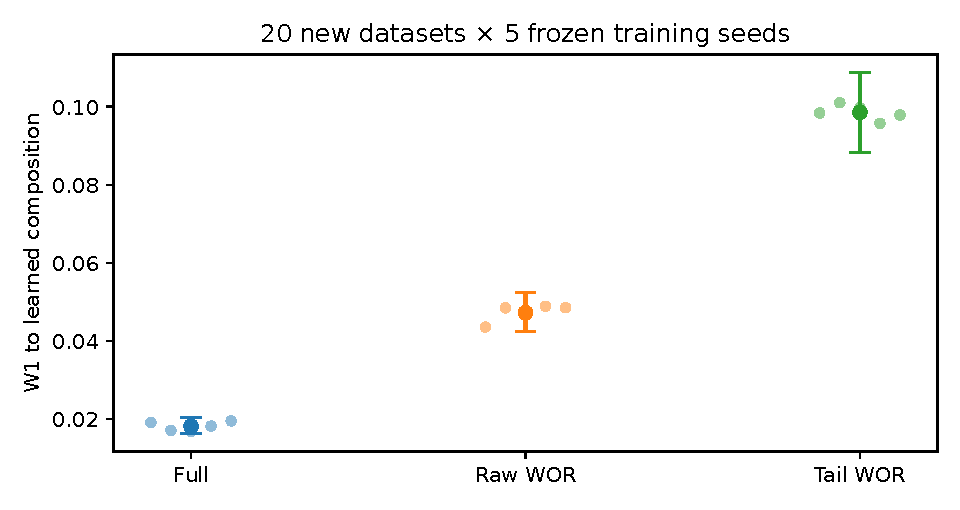
\includegraphics[width=0.82\linewidth]{figures/solid_heldout.pdf}
 \caption{New learned-density replication. Large points show overall means with crossed-bootstrap 95\% intervals; five smaller points show the means for individual training seeds, each averaged over the same 20 datasets. Raw WOR has an infinite population normalizer throughout, whereas Full and Tail WOR are finite throughout.}
 \label{fig:solid-heldout}
\end{figure}

\subsection{Sampling on both sides of a validity threshold}
The rechecked critical batch sizes are 60 and 59 for the Gaussian and ordinary-mixture families at $K=512$ and 2048, respectively, and 18 and 17 for the weak mixture. In each of these six settings, the certificate is infinite at $M_{\rm crit}-1$ and finite at $M_{\rm crit}$. Both full weighting and $M=4$ tail control are finite. Table~\ref{tab:solid-boundary} includes every setting, with intervals in Figure~\ref{fig:solid-boundary}.

\begin{table}[H]
 \centering
 \caption{Mean marginal W1 across ten new sampling seeds near the certificate boundary. Below and At use raw WOR with $M=M_{\rm crit}-1$ and $M=M_{\rm crit}$, respectively. Below is infinite in every row; the other three conditions are finite. Tail uses $M=4$.}
 \label{tab:solid-boundary}
 \begin{tabular}{lrrrrrr}
 \toprule
 Family & $K$ & $M_{\rm crit}$ & Full & Below & At & Tail\\
 \midrule
 Gaussian & 512 & 60 & 0.01854 & 0.02385 & 0.01543 & 0.01911\\
 Gaussian & 2048 & 59 & 0.01965 & 0.01777 & 0.02172 & 0.02107\\
 Mixture & 512 & 60 & 0.86302 & 0.81897 & 0.68900 & 1.43500\\
 Mixture & 2048 & 59 & 0.85092 & 0.85712 & 0.66242 & 1.52086\\
 Weak mixture & 512 & 18 & 0.04455 & 0.03798 & 0.03498 & 0.03523\\
 Weak mixture & 2048 & 17 & 0.02948 & 0.03142 & 0.03945 & 0.03397\\
 \bottomrule
 \end{tabular}
\end{table}

Observed accuracy changes in both directions across the validity boundary. For the ordinary mixture at $K=2048$, the At-minus-Below difference is $-0.19469$, with paired interval $[-0.33562,-0.05965]$. For the weak mixture at the same resolution, it is $0.00802$, with interval $[0.00061,0.01784]$. These are descriptive intervals without adjustment across the six boundary comparisons. The certificate classifies existence of the population update; it does not require a monotone change in finite-particle endpoint error at the threshold.

\begin{figure}[H]
 \centering
 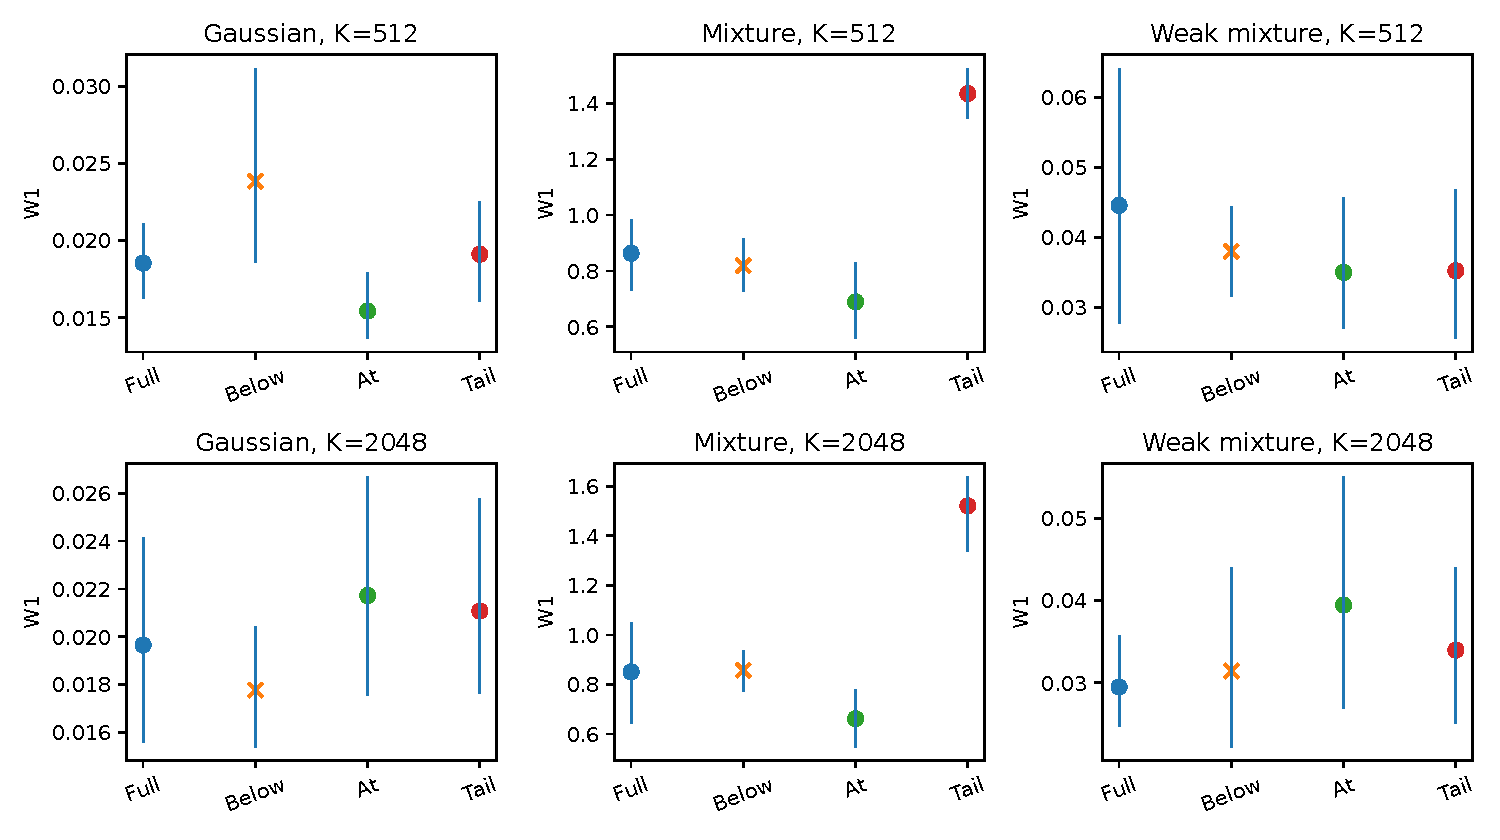
\includegraphics[width=\linewidth]{figures/solid_boundary.pdf}
 \caption{All six boundary comparisons, each with ten sampling seeds. Points show means and vertical bars show bootstrap 95\% intervals. Circles denote finite normalizers and crosses infinite ones. Panel-specific vertical scales retain the differences in error magnitude between families.}
 \label{fig:solid-boundary}
\end{figure}

\subsection{Sensitivity to an imperfect tail control}
Figure~\ref{fig:solid-tail-sensitivity} reports all 66 deterministic perturbations. Every tested perturbation with $|\delta|\le0.1$ is finite for all three families and both grids. At $\delta=\pm0.25$, the Gaussian and ordinary-mixture certificates are infinite on both grids, whereas the weak-mixture certificates remain finite. There are 58 finite and eight infinite configurations; no zero-denominator case is classified. These grid values demonstrate tolerance to the specified perturbations in the tested models, without establishing a uniform robustness interval for arbitrary factors or score errors.

\begin{table}[H]
 \centering
 \caption{Mean marginal W1 under multiplicative control-variance error, with the target held fixed. Each entry averages ten seeds at $K=512$, $P=8192$, $M=4$, with replacement. Every displayed setting has a finite certificate.}
 \label{tab:solid-tail-error}
 \begin{tabular}{lrrr}
 \toprule
 Family & $\delta=-0.1$ & $\delta=0$ & $\delta=0.1$\\
 \midrule
 Gaussian & 0.01974 & 0.01845 & 0.01882\\
 Mixture & 1.14131 & 1.18388 & 1.35780\\
 Weak mixture & 0.03086 & 0.03385 & 0.03260\\
 \bottomrule
 \end{tabular}
\end{table}

Finite certificates do not eliminate sensitivity of sampling error. For the ordinary mixture, the $\delta=0.1$ minus $\delta=0$ difference is $0.17392$, with a descriptive paired interval of $[0.00940,0.36340]$. The complete seed-level results and all six perturbation-comparison intervals are retained, including intervals spanning zero.

\begin{figure}[H]
 \centering
 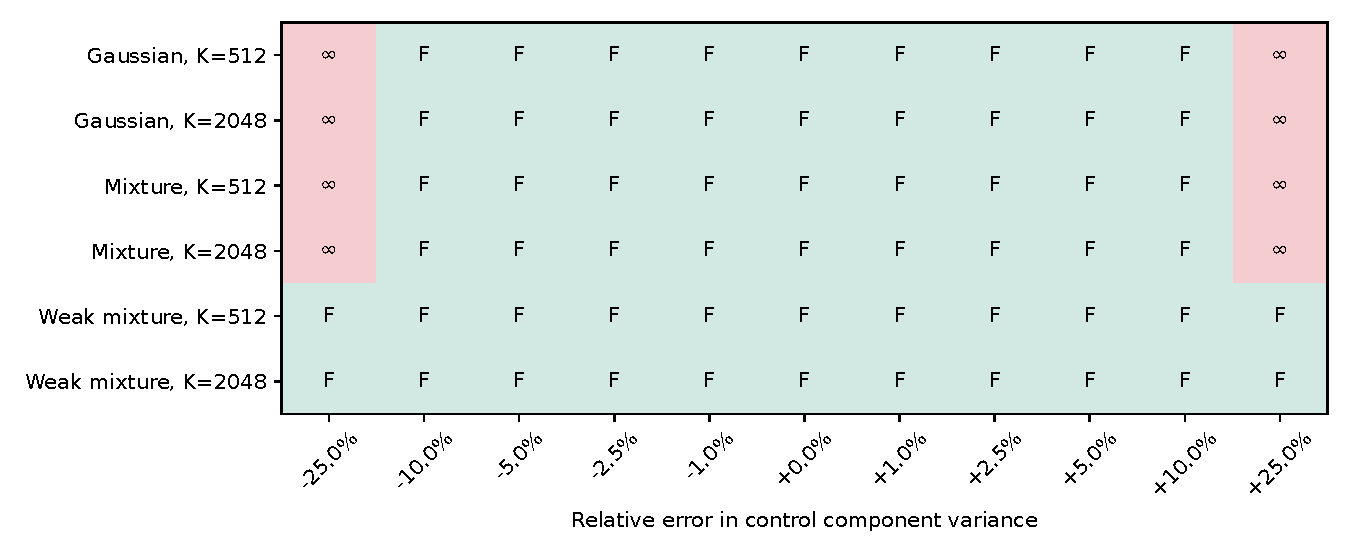
\includegraphics[width=\linewidth]{figures/solid_tail_sensitivity.pdf}
 \caption{Strict-domain certificates for every tested control-variance perturbation. F denotes a finite normalizer and $\infty$ an infinite one. Columns are the discrete tested values of $\delta$, not a continuous parameter grid or an assertion about untested values.}
 \label{fig:solid-tail-sensitivity}
\end{figure}

\subsection{Independent verification and remaining scope}
All 630 sampling cells completed with a zero launcher exit status, and every original particle array is retained. We reload all five checkpoints, regenerate the 20 datasets, and verify the 100 learned parameter sets and their consistency across methods. Independent SciPy reference calculations use 131,073 points on $[-16,16]$, with a separately implemented Gaussian-mixture density. These checks cover 103 learned/oracle parameter settings and their corresponding true-posterior references. Independent recomputation checks W1, KS, means, variances, and positive-coordinate masses for every cell. The maximum W1 discrepancy against the original records is $1.61\times10^{-6}$. A separate vectorized recursion checks 333 sampling-certificate configurations and all 66 sensitivity configurations, including failure steps. Source hashes, checkpoint hashes, complete cell manifests, and the recovered raw-file hashes are retained.

This replication strengthens evidence within the controlled simulator and explicit Gaussian-tail model class. It introduces no additional training replicates and provides no validation on a real scientific inverse problem, arbitrary neural scores, or non-diagonal tails. The new data support the distinction between population validity and finite-particle accuracy; they do not establish general speed--accuracy superiority for tail control.

\end{document}
